\chapter{IRK metodo sinplektikoen bidezko eguzki-sistemaren integrazioa}


\section{Sarrera.}
  


Kapitulu honen jatorrizko helburua, aurreko  bi kapituluetan landutako IRK metodo sinplektikoen inplementazioak (\ref{chap:IRK-PF}~kapituluan puntu-finkoaren iterazioan oinarritutakoa eta \ref{chap:IRK-NEW}~kapituluan Newton sinplifikatuaren iterazioan oinarritutakoa) eguzki sistemaren zenbakizko integraziorako aplikatzea da.  Zenbait proba egin ondoren, ondorioztatu dugu Newton-en iterazio sinplifikatuan oinarritutako inplementazioa baino eraginkorragoa dela kasu  honetan puntu finko partizionatuan oinarritutako inplementazioa. Bestalde, eguzki-sistemaren simulaziorako ekuazio diferentzialen sistemak ekuazio Kepleriarren perturbazio gisa har daitezkeenez, honetaz baliatzen saiatzea erabaki dugu IRK metodo sinplektikoen bidezko zenbakizko integrazio eraginkorrak lortze aldera.

Helburu horrekin,  kapitulu honetan ekuazio diferentzial Kepleriarren perturbazio gisa har daitezkeen ekuazio diferentzialen sistemen zenbakizko integraziorako metodo berri bat proposatuko dugu. Gure metodo berria ondorengo ideian  oinarritzen da: fluxu Kepleriarrean oinarritutako aldagai aldaketa bat aplikatuz, aldagai berrietan idatzitako ekuazio diferentzialetatik alde Kepleriarra desagerrarazi, eta dagokien ekuazio sistemari IRK metodo sinplektiko bat aplikatzea.


Proposatuko dugun metodoa, sinplektikoa eta denborarekiko simetrikoa da, neurri batean, splitting metodoen antzekoa. Aldagai berriekiko ekuazio diferentzialak, magnitude txikiko balioak hartzen dituzte eta honek, hainbat abantaila izango ditu. Lehenik, eguzki-sistemaren problemaren trunkatze errore nagusiena ezabatzen dugunez, urrats luzera handiagoak erabili ahal izango ditugu. Bigarrenik, aldagai berriekiko ekuazio diferentzialen zenbakizko ebazpenean, biribiltze erroreen eragina txikiagoa izango da (batura konpentsatuaren algoritmoan bit gutxiago galduko ditugu). Hirugarrenik, puntu-finkoaren iterazioek konbergentzia azkarragoa izango dute (aldagai berrietako ekuazioen espresioen deribatu partzialak tamaina txikikoak direlako).

 Lehenengo, problema perturbatuetarako oinarrizko metodoa azalduko dugu,  perturbatu gabeko zatiaren fluxuaren bidezko aldagai aldaketan oinarritutako   integrazio metodoaren zehaztapenak emango ditugularik.
Ondoren, aipatutako integrazio eskema orokorra  hainbat ekuazio Kepleriarren perturbazio gisa har daitezkeen sistemetarako aplikatzeko zenbait xehetasun emango ditugu.  Azkenik,  metodo berri hau eguzki-sistemaren eredu sinplifikatu baterako aplikatuko dugu, eta ezagutzen diren hainbat metodo esplizitu sinplektikorekin (doitasun altutarako splitting eta konposizio metodoekin) konparatuko dugu.
Aipatutako eguzki-sistemaren eredu sinplifikatua, eguzkia, zortzi planetak, eta Pluton hartzen dituen 10 gorputzeko eredu Newtoniarra da, koordenatu Heliozentriko kanonikotan adierazia  (ikus ~\ref{erans:B2}~eranskina).

 
\section{Sistema perturbatuetarako integrazio metodo simetriko mota orokor bat}
 \label{s:metodoberria}


 Demagun honako ekuazio diferentzialen sistema dugula,
\begin{align}
\begin{split}
\label{eq:pertEDA}
&\frac{du}{dt} = k(u) + g(u,t), \quad  u(t_0) = u_0 \in \mathbb{R}^D
\end{split}
\end{align}
non $g(u,t)$ perturbazio gisa hartzen dugun. Demagun gainera pertubatu gabeko zatia,
\begin{equation}
\label{eq:unpert}
\frac{du}{dt} u = k(u),
\end{equation}
%
edozein hasierako baliotarako zehazki ebazteko gai garela, alegia, bere $t$-fluxua $\varphi_{t}: \mathbb{R}^{D} \to \mathbb{R}^{D}$
 zehazki ebazteko gai garela. Gogora dezagun fluxuaren definizioz,
 \begin{equation}
 \label{eq:fluxudef}
\frac{\partial}{\partial t} \varphi_{t}(u) \equiv k(\varphi_{t}(u))
\end{equation}
%
identitatea daukagula.

Esate baterako,   (\ref{eq:unpert}) sistema Kepleriarra izan liteke, hau da,
\begin{equation}
\label{eq: hamkepler}
H(q,p)=\frac{p^2}{2m}-\frac{\mu}{\|q\|},
\end{equation}
funtzio Hamiltondarrari dagokion EDA sistema, non $u=(q,p) \in \mathbb{R}^{6}$, eta
$m$ eta $\mu$ parametro konstanteak diren. (Ikus xehetasun gehiagorako \ref{erans:B1}~eranskina.)
Eguzki-sistemaren simulaziorako aplikatzerakoan, perturbatu gabeko (\ref{eq:unpert}) sistema hainbat ekuazio Kepleriar independentez osatuta egongo da, eta $g(u,t)$ perturbazioan, ekuazio Kepleriar horien arteko interakzioa biltzen dituen gaiak izango ditugu. (Xehetasun gehiagorekin azalduko dugu kasu hau \ref{s:Keplerrak}~atalean).


Gure metodoaren $h$ luzerako urrats bat definitzeko,  $u_0$ hasierako balioa ezaguturik (\ref{eq:pertEDA}) problemaren $u(t)$ soluzioaren $t=t_0+h$ uneko balioa hurbiltzeko prozedura zehaztu behar dugu. Horretarako,  (\ref{eq:pertEDA})  sistemari aldagai aldaketa bat aplikatuko diogu, eta aldagai berrietan idatzitako problema ebatziko dugu IRK metodo sinplektiko baten bidez. Aplikatuko dugun aldagai aldaketa honakoa da
\begin{equation*}
u = \varphi_{t-t_0-h/2}(U) \quad \to \quad U = \varphi_{-t+t_0+h/2}(u).
\end{equation*}
%
Aldagai berrietan idatzitako ekuazio diferentzialen sistema lortzeko, honakoa egingo dugu,
\begin{align}
\begin{split}
&\frac{d}{dt}u(t) = \frac{d}{dt}\left(\varphi_{t-\tau}(U(t))\right),
\end{split}
\end{align}
%
non $\tau = t_0+h/2$ den.
Eskuin aldeari katearen erregela aplikatuz, eta ezker alderako (\ref{eq:pertEDA}) eta aldagai aldaketa kontutan hartuz, eta $U(t)$ idatzi ordez $U$ jarriz,
\begin{align}
\begin{split}
&k\left(\varphi_{t-\tau}(U)\right) + g\left(\varphi_{t-\tau}(U),t \right) = \frac{\partial}{\partial t} \varphi_{t-\tau}(U) + \varphi'_{t-\tau}(U) \frac{d}{dt}U,
\end{split}
\end{align}
non $\varphi'_{t-\tau}(U)$ espresioak fluxuaren $U$ aldagaiekiko matrize Jacobiarra adierazten duen. Ondoren, (\ref{eq:fluxudef}) identitatea aplikatuz, honakoa lortzen dugu
\begin{align}
\begin{split}
&g\left(\varphi_{t-\tau}(U),t \right) =   \varphi'_{t-\tau}(U) \frac{d}{dt}U,
\end{split}
\end{align}
%
eta beraz, jatorrizko (\ref{eq:pertEDA}) ekuazio diferentzialen problema $U$ aldagai berritan idaztea lortu dugu, hau da,
\begin{align}
\begin{split}
\label{eq:pertEDAU}
&\frac{d}{dt} U = \left(\varphi'_{t-\tau}(U)\right)^{-1} g\left(\varphi_{t-\tau}(U),t \right), \quad U(t_0) = U_0,
\end{split}
\end{align}
%
non
\begin{equation*}
U_0 = \varphi_{h/2}(u_0)
\end{equation*}
%
den.  Hortaz, (\ref{eq:pertEDAU}) problemarako $t=t_0$ unetik $t=t_1:=t_0 + h$ unera IRK metodoarekin integratuz, $U_1 \approx U(t_1)$ lortuko dugu, eta
aldagai aldaketari buelta emanez $u(t_1) = \varphi_{h/2}(U(t_1))$ lortzen dugunez, $u_1 \approx u(t_1)$ kalkulatzeko,
\begin{equation*}
u_1 = \varphi_{h/2}(U_1)
\end{equation*}
%
egingo dugu.

Orain arte, metodoaren lehen urratsa nola eman deskribatu dugu, baina $t=t_0$ uneko $u(t_0)$ egoeratik $t=t_1$ uneko $u(t_1)$ egoeraren $u_1$ hurbilpena lortzeko prozedura berbera erabil dezakegu, $j=1,2,3,\ldots$ indizetarako, $t=t_{j}$ uneko $u(t_j)$ egoeraren $u_j$ hurbilpenetik $t=t_{j+1}:= t_{j}+h$ uneko $u(t_{j+1})$ egoeraren $u_{j+1}$ hurbilpena lortzeko. Kontutan hartu behar da urrats bakoitzean aplikatu beharreko aldagai aldaketa  desberdina dela, alegia, $(j+1)$. urratsean, $U$ aldagai berriak jatorrizko $u$ aldagaiekin $u = \varphi_{t-\tau_j}(U)$ moduan erlazionaturik izango ditugula, non $\tau_j = t_j + \frac{h}{2}$ den. Urrats bakoitzean aplikatutako aldagai aldaketa bereizteko, $(j+1)$. urratseko aldagai berria $U^{j+1/2}$ gisa adieraziko dugu.

 Horrela, $(j+1)$. urratsean, $u_j \approx u(t_j)$ emanik, lehenik dagokion aldagai berriaren balioa kalkulatuko dugu,
\begin{equation*}
U^{j+1/2}_j = \varphi_{h/2}(u_j)
\end{equation*}
%
ondoren, gure IRK metodoaren $h$ luzerako urrats bat aplikatuko dugu ondorengo problemarako,
\begin{align}
\begin{split}
\label{eq:pertEDAUj}
&\frac{d}{dt} U^{j+1/2} = \left(\varphi'_{t-\tau_j}(U^{j+1/2})\right)^{-1} g\left(\varphi_{t-\tau_j}(U^{j+1/2}),t \right), \quad U^{j+1/2}(t_j) = U^{j+1/2}_j,
\end{split}
\end{align}
%
$U^{j+1/2}_{j+1} \approx U^{j+1/2}(t_{j+1})$ hurbilpena lortuz, eta azkenik, metodoaren urratsa bukatzeko,
%
\begin{equation*}
u_{j+1} = \varphi_{h/2}(U^{j+1/2}_{j+1})
\end{equation*}
%
kalkulatuko dugu.  Laburbilduz:
%
\begin{align*}
   &   \quad U^{j+1/2}_j \quad \quad \quad \quad \stackrel{\Longrightarrow}{IRK(\ref{eq:pertEDAUj})}  & U^{j+1/2}_{j+1}&  &\\
  & \nearrow \varphi_{\frac{h}{2}}(u_j) &            & \searrow \varphi_{\frac{h}{2}}(U^{j+1/2}_{j+1})& \\
u_j &                  &    &\quad \quad \quad  u_{j+1}
\end{align*}
%
Urrats bakoitzerako aldagai aldaketa definitzeko erabiltzen dugun erreferentziazko $\tau_j=t_j+h/2$ unea $t_j$ eta $t_{j+1}$ balioen erdigunea aukeratu dugu. Hori horrela egiteak badu arrazoi bat: urratsa bere osotasunean denborarekiko simetrikoa da, aplikatutako IRK metodoa ere denborarekiko simetrikoa da: Kasu horretan, ikus daiteke aurrera $h$ luzerako urratsa ematea $-h$ luzerako urratsa ematearekin desegiten dela.


Metodoaren integrazio eskema orokorra \ref{fig:proiekzioa0}~irudian laburtu dugu.
\begin{figure} [h!]
{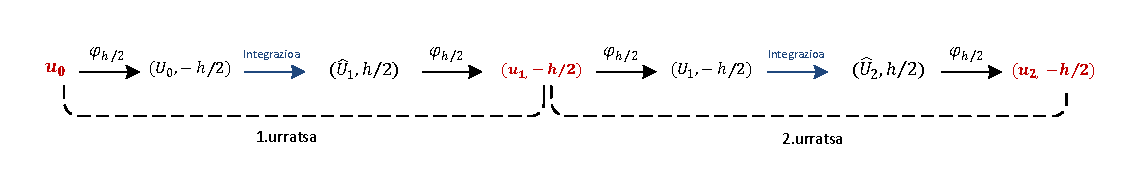
\includegraphics [width=16cm, height=4cm] {proiekzioa11}}
\caption{\small Metodoaren integrazio eskema orokorra}
\label{fig:proiekzioa0}
\end{figure}
%


Nolabait, guk proposatutako metodoa splitting metodoen antzekoa da, bereziki, bigarren ordenako (\ref{eq:stverlet}) Strang-en splitting metodoaren antzekoa. Gogora dezagun Strang-en metodoa era honetan aplikatzen dela: $\varphi_{h/2}$ fluxua aplikatu, perturbazioari soilik dagokion ekuazioaren soluzioa kalkulatu $h$ urrats luzerarako, eta berriz   $\varphi_{h/2}$  fluxua aplikatu. Fluxuaren aldagai aldaketarekin, gauza bera egiten ari gara, baina  $\varphi_{h/2}$ fluxuaren bi aplikazioen artean egiten duguna konplexuagoa izatearen truke,  bigarren ordenako metodoa lortu ordez, aldagai berrietarako aplikatzen dugun IRK metodoaren ordena bereko metodoa lortzen dugu.


Inplementazioaren eraginkortasunaren aldetik, integrazioaren urrats guztietan ez baditugu emaitzak itzuli behar, bi urratsen arteko, $\varphi_{h/2}$ fluxuaren bi konputazioak, $\varphi_{h}$ fluxuaren konputazio bakarrarekin konputatuko dugu. Esate baterako, \ref{fig:proiekzioa0} irudian, $u_1$ behar ez bada, zuzenean kalkula daiteke $U^{3/2}_1 = \varphi_{h}(U^{1/2}_1)$, fluxua kalkulatzen duen funtzioari dei bakarra eginez, bi dei egin beharrean.



Metodoaren urrats bakoitza sinplektikoa da (\ref{eq:pertEDA}) sistema perturbatua eta perturbatu gabeko (\ref{eq:unpert}) sistema biak Hamiltondarrak baldin badira, eta aldi berean, (\ref{eq:pertEDAUj}) problemaren zenbakizko ebazpenerako  IRK sinplektikoa erabiltzen bada. Hain zuzen, kasu horretan $\varphi_{h/2}$ sinplektikoa da, eta horren ondorioz (\ref{eq:pertEDAUj}) problema Hamiltondarra denez, IRK sinplektikoaren urrats bakoitza sinplektikoa izango da, eta beraz, metodoaren $u_j \to u_{j+1}$ urrats bakoitza ere sinplektikoa izango da.

Azkenik,  bai (\ref{eq:pertEDA}) sistema perturbatuak eta bai perturbatu gabeko (\ref{eq:unpert}) sistemak $I(u)$ inbariante bera onartzen badute, antzera ondoriozta daiteke   (\ref{eq:pertEDAU}) problemarako ere $I(U)$ inbariantea dela, eta beraz inbariante hori koadratikoa baldin bada, eta IRK metodoa sinplektikoa baldin bada, gure metodoak inbariante hori konstante mantenduko duela.

Urrats bakoitzari dagokion aldagai berrietan idatzitako (\ref{eq:pertEDAU}) sistemaren eskuinaldea balioztatzeari dagokionean, sistema perturbatu gabea Hamiltondarra baldin bada, Jacobiarraren alderantzizkoa kalkulatzea ekidin daiteke.  Hain zuzen, bere $t$-fluxua sinplektikoa denez,  $(\varphi'_{t}(U))^tJ\varphi'_{t}(U)= J$ propietatea betetzen du fluxuak $\forall(t,U) \in \mathbb{R}^{D+1}$, non
\begin{equation*}
 J=\left(\begin{array}{cc}
   \ 0 & \ -I \\
     I & \ 0  \\
\end{array}\right)
\end{equation*}
den, eta  ondorioz, $G \in \mathbb{R}^D$ emanik
%
\begin{align}
\begin{split}
\label{eq:hamEDAU2}
& (\varphi'_{t-\tau}(U) )^{-1} G = J^{-1}(\varphi'_{t-\tau}(U))^{T} J G.
\end{split}
\end{align}
%
Beraz,  (\ref{eq:pertEDAU})  sistemaren eskuinaldeko $F$ espresioa balioztatzeko, hurrengo moduan egin daiteke:
\begin{itemize}
\item $u=\varphi_{t-\tau}(U)$,
\item $G=g(u,t)$ balioztatu, eta ondoren $\widehat G=J G$,
\item $\widehat F = \varphi'_{t-\tau}(U)^{T} \widehat G$,
\item $F = J^{-1} \widehat F$.
\end{itemize}
%
Goiko algoritmo horretan, hirugarren atala modu eraginkorrean egin daiteke deribazio automatikoko teknikak erabiliz, lehen ataleko kalkuluan erabilitako zenbait tarteko aldagai berrerabiliz gero.


Azkenik, aplikazioetan ohikoa izango da perturbazioari dagokion espresioak balio txikiak hartzea. Kasu horretan biribiltze erroreen eragina txikitzeko komenigarria da, doitasun mistoa erabiltzea: Oinarrizko doitasunean aplikatzea (batura konpentsatuarekin) IRK metodoa (\ref{eq:pertEDAUj}) problemari, baina doitasun altuagoan aplikatzea  \ref{fig:proiekzioa0}~irudian azaltzen diren $\varphi_{h/2}$ fluxuak (edo $\varphi_{h}$ fluxua, irteerarik behar ez den kasuan).


\section{Sistema Kepleriarren perturbaziotarako aplikazioa}
\label{s:Keplerrak}

Goian aipatu bezala, eguzki-sistemaren simulaziorako aplikatzerakoan,  mugimenduaren ekuazioak hainbat ekuazio Kepleriar independenteren
perturbazio gisa har daitezke.  Horretan oinarritzen dira hain zuzen, eguzki-sistemaren simulaziorako aplikatzen diren splitting metodoak (\ref{s:KonSpl}~atala).
Era berean, \ref{s:metodoberria}~atalean garatutako metodoak aplika daitezke kasu horretan.

Demagun problemaren alde Kepleriarren kopurua $n$ dela, eta
\begin{equation*}
u=(q_1,v_1,\ldots,q_n,v_n,w) \in \mathbb{R}^{D},
\end{equation*}
 non $w \in \mathbb{R}^{D-6 n}$, eta (\ref{eq:pertEDA}) moduko sistemaren zenbakizko integrazioa burutu nahi dugula  \ref{s:metodoberria}~atalean garatutako metodorekin, perturbatu gabeko (\ref{eq:unpert}) sistema $(q_i,v_i) \in \mathbb{R}^{6}$ aldagaietarako sistema Kepleriar independentez osatuta dagoelarik. Zehazkiago, demagun
%
\begin{equation}
\label{eq: n-pertEDA}
k(u) =
\left(\begin{array}{c}
               v_1 \\
             \displaystyle  - \frac{\mu_1 \ q_1}{\|q_1\|^3}\\
               v_2 \\
                \displaystyle  - \frac{\mu_2 \ q_2}{\|q_2\|^3}\\
                \vdots \\
                v_n\\
                \displaystyle  - \frac{\mu_n \ q_n}{\|q_n\|^3}\\
                               0
\end{array}\right),
\end{equation}
%
non $\mu_j>0$ ($j=1,\ldots,n$) diren.

Kasu horretan, (\ref{eq:unpert}) sistemaren $t$-fluxua $u=(q_1,v_1,\ldots,q_n,v_n,w)$ punturako aplikatzeko, $(q_j,v_j)$ bakoitzerako dagokion fluxu Kepleriarra
aplikatu beharko dugu, eta $w$ bere horretan utzi. Zehazkiago,
 $u = \varphi_{t-\tau}(U)$ moduko aldagai aldaketa, $U=(Q_1,V_1,\ldots,Q_n,V_n,W)$ izanik, horrela definiturik egongo da,
%
\begin{align}
\label{eq:aldfl2}
\begin{split}
u_j&= \varphi_{t-\tau}^{[\mu_j]}(U_j), \quad  j=1,\dots,n, \quad w = W,
\end{split}
\end{align}
%
non, $j \in \{1,\ldots,n\}$ bakoitzerako, $\varphi_{t-\tau}^{[\mu_j]}:\mathbb{R}^6 \to \mathbb{R}^6$ dagokion sistema Kepleriarraren $(t-\tau)$-fluxua den. (Ikus ?~eranskina hau praktikan kalkulatzearen inguruko xehetasunetarako.)


Bestalde,  aldagai berritan idatzitako (\ref{eq:pertEDAU}) ekuazio diferentzialen sistemaren eskuin aldeko espresioa balioztatzeko, \ref{s:metodoberria}~atalaren amaieran azaltzen den algoritmoa aplikatzeko, $\widehat G \in \mathbb{R}^D$ emanik,  $\widehat F = \varphi'_{t-\tau}(U)^{T} \widehat G$ kalkulatu behar dugu.
Hori egiteko, demagun $\widehat G = (\widehat G_1,\ldots,\widehat G_n,\widehat G_{n+1})$ eta  $\widehat F = (\widehat F_1,\ldots,\widehat F_n,\widehat F_{n+1})$ direla. Notazio horrekin,
\begin{equation*}
\widehat F = \varphi'_{t-\tau}(U)^{T} \widehat G
\end{equation*}
 kalkulatzeko, nahikoa izango da honakoa egitea,
\begin{equation*}
\widehat F_j =  \varphi^{[\mu_{j}]'}_{t-\tau}(U_j)^{T} \widehat G_j, \quad j=1,\ldots,n, \quad \widehat F_{n+1} = \widehat G_{n+1}.
\end{equation*}



\section{Zenbakizko esperimentuak.}
\label{s:7espmt}

Zenbakizko esperimentuetarako, puntu-finkoaren iterazioan oinarritutako Gauss metodoaren inplementazioa (\ref{chap:IRK-PF}~kapitulua) erabili dugu. Lehenengo, Gauss metodoaren bi bertsio konparatu ditugu: aldagai aldaketarik gabeko integrazioa eta aldagai aldaketa aplikatutako integrazioa. Kepler fluxuan oinarritutako aldagai aldaketarekin integrazioaren abantaila argia denez, hurrengo esperimentuetarako aldagai aldaketa aplikatutako integrazioa bakarrik hartu dugu kontutan.  
 
$s=6,8,9,16$ ataletako Kepler-en fluxuan oinarritutako aldagai aldaketa aplikatutako Gauss metodoen arteko metodo eraginkorrena aukeratu dugu, \emph{CO1035} konposizio eta \emph{ABAH1064} splitting  metodoekin konparatzeko.

Gauss metodoen konputaziorako, $64$-biteko (\emph{double}) eta $80$-biteko (\emph{long double}) doitasunak nahasi ditugu. Konputazioaren zati nagusiena, $64$-biteko doitasunean egin dugu eta proiekzioa kalkulatzeko, $80$-biteko doitasuna aplikatu dugu. Era honetan, modu merkean soluzioaren doitasuna hobetzea lortu dugu.

Gauss metodoaren exekuzio sekuentziala eta paraleloak egin ditugu. $s$ atalen funtzioen balioztapena, 
\begin{align*}
F_{n,i}=f(Y_{n,i}), \ i=1,\dots,s,
\end{align*}      
independenteak dira eta paraleloan kalkula daitezke. $s=8$ metodoaren integrazio paraleloak egin ditugu eta hari kopurua $2$ aplikatu dugu. 

\subsection{Problemak.}


9-planeten problema (\ref{sss:9body}~atala) erabili dugu integrazioetarako. Hasierako balioak \emph{DE-430} efemerideen artikulutik hartu ditugu: planeten masak  \ref{tab:9bodymas}~taulan laburtu ditugu; eta hasierako kokapen eta abiadurak \ref{tab:9bodyhas}~taulan aurki daitezke.

Koordenatu heliozentrikoei dagokien  Hamiltondar sistema (\ref{eq:nbodyHel}),
\begin{align*}
&H(q,p)=H_K(q,p)+H_I(q,p),
%&H(q,p)=\sum\limits_{i=1}^{N}\bigg(\frac{\|P_i\|^2}{2 \mu_i} -\frac{G m_0 m_i}{\|Q_i\|}\bigg)+H_I(q,p)
\end{align*}
integratu dugu. $H_K(q,p)$ mugimendu Kepleriarrari dagokion Hamiltondarraren aldea da  eta $H_I(q,p)$, perturbazioei dagokien Hamiltondarraren aldea da. 
%Kepler-en fluxuan oinarritutako aldagai aldaketaren bidez, alde Kepleriarra ekuazioetatik desagerrarazten dugu.    

Integrazioen tartea, $t_{end}=10^6$ egunetakoa da eta zenbakizko integrazioetan, $h$-ren balio ezberdinak erabili ditugu. $s=6$ metodoarentzat urrats luzerak aukeratu ditugu eta gainontzeko metodoentzat, $s$-atalen araberako urrats luzera proportzionalak finkatu ditugu:
\begin{align*}
&s=6: \quad  \ \ h=2^{k/4}, \ k=4,\dots,28, \\
&s=8: \quad  \ \ (8/6)h, \\
&s=9: \quad  \ \ (9/6)h, \\
&s=16: \quad (16/6)h. \\
\end{align*} 

Zenbakizko esperimentuetarako, aldagai aldaketa planeta guziei aplikatzea erabaki dugu. $9$-planeten probleman, gorputz kopurua txikia denez,  Kepler fluxuaren gainkarga esanguratsua da eta  barne-planetei bakarrik aplikatzea, eraginkorragoa izan daiteke. Baina, gorputz gehiago kontsideratzen baditugu (esaterako Ilargia eta asteroide nagusienak) edo eguzki-sistemaren eredu konplexuagoetan (esaterako erlatibitate efektua gehitzerakoan), perturbazio aldearen konputazioa nagusituko da eta Kepler fluxuaren kalkuluak pisua galduko luke. 


\subsection*{Gauss metodoen eraginkortasuna.}


\ref{fig:esp81a}~irudian, $s=6$ ataletako Gauss metodoaren bi bertsioen eraginkortasunak konparatu ditugu: aldagai aldaketarik gabeko integrazioa eta aldagai aldaketa aplikatutako integrazioa. Aldagai aldaketarik gabeko integraziorako, puntu-finkoaren iterazio partizionatua eta interpolazio bidezko hasieraketa aplikatu dugu. Ekuazio diferentzialen ebaluazioen konparaketan, aldagai aldaketa aplikatutako integrazioa, nabarmen eraginkorragoa da. Eredu sinplearen integrazioen exekuzio denboren konparaketan, aldea txikiago da, baina orduan eta eredu konplexuagoa izan abantaila handituz joango da.   

\begin{figure}[h!]
\centering
\begin{tabular}{c c}
\subfloat[ Gauss metodoak (FCN).]
{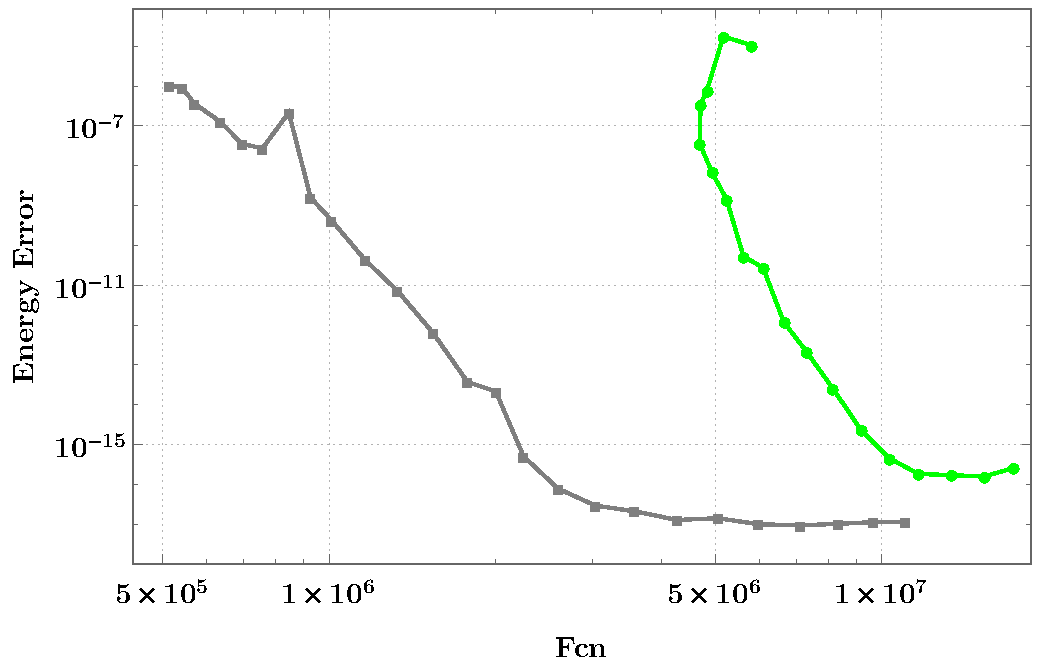
\includegraphics[width=.45\textwidth]{esperimentua801}}
&
\subfloat[ Gauss metodoak (CPU).]
{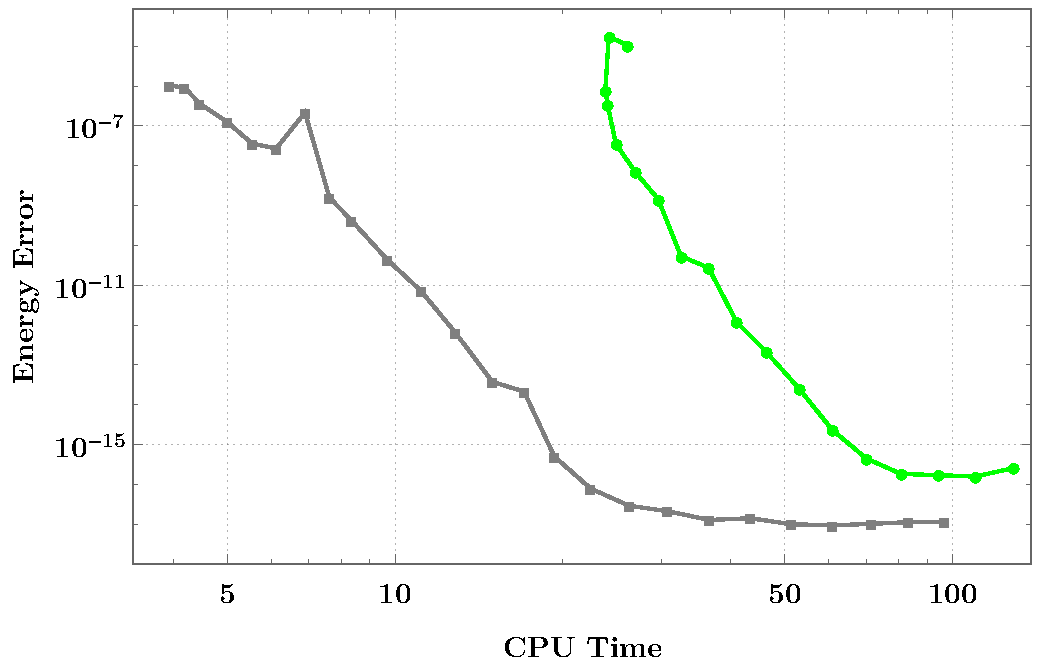
\includegraphics[width=.45\textwidth]{esperimentua802}}
\end{tabular}
\caption[Puntu-finkoaren eraginkortasun grafikoak]{\small 
Eraginkortasun grafikoak eskala logaritmiko bikoitzean irudikatu ditugu. Ardatz bertikalean, energiaren errore erlatibo maximoa eman dugu. (a) irudian, ekuazio diferentzialen ebaluazio kopuruarekiko (FCN) eraginkortasuna neurtu dugu. (b) irudian, CPU denborarekiko eraginkortasuna neurtu dugu. Irudi bakoitzean, Gauss metodoaren $s=6$ ataletako bi bertsio konparatu ditugu: aldagai aldaketa gabe berdez eta aldagai aldaketa aplikatuta grisez. }
\label{fig:esp81s}
\end{figure}

Jarraian, $s=6,8,9,16$ ataletako metodoen eraginkortasuna aztertu dugu. \ref{fig:esp81a}~irudian, diferentzialen ebaluazio kopuruarekiko (\emph{FCN}) eta \ref{fig:esp81s}~irudian, \emph{CPU}-denborarekiko (exekuzio paraleloetan \emph{Wall time}) erakutsi dugu. \emph{FCN}-rekiko eraginkortasuna, metodoak problema erreal batean nola jokatuko luke erakusten digu eta \emph{CPU}-rekiko  eraginkortasuna, problema zehatz honetarako gertatzen dena azaltzen digu.


\begin{figure} [h!]
\centerline{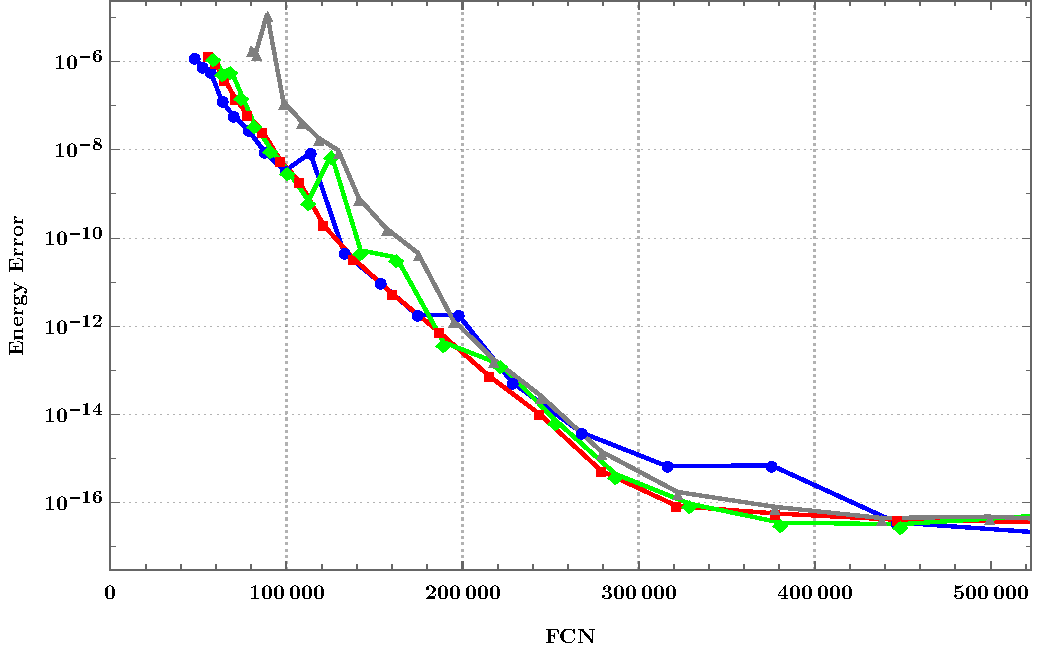
\includegraphics [width=8cm, height=6cm] {esperimentua812}}
\caption[Gauss metodoen eraginkortasun konparaketa (FCN)]{\small Eraginkortasun grafikoa eskala logaritmiko bikoitzean irudikatu dugu. Ardatz bertikalean, energiaren errore erlatibo maximoa eman dugu eta ardatz horizontalean, ekuazio diferentzialen ebaluazio kopurua (FCN). Gauss metodoaren $s$ ataletako lau integrazio konparatu ditugu: $s=6$  urdinez, $s=8$ gorriz, $s=9$ berdez, eta $s=16$ grisez}
\label{fig:esp81a}
\end{figure} 


\begin{figure}[h!]
\centering
\begin{tabular}{c c}
\subfloat[ Exekuzioa sekuentziala.]
{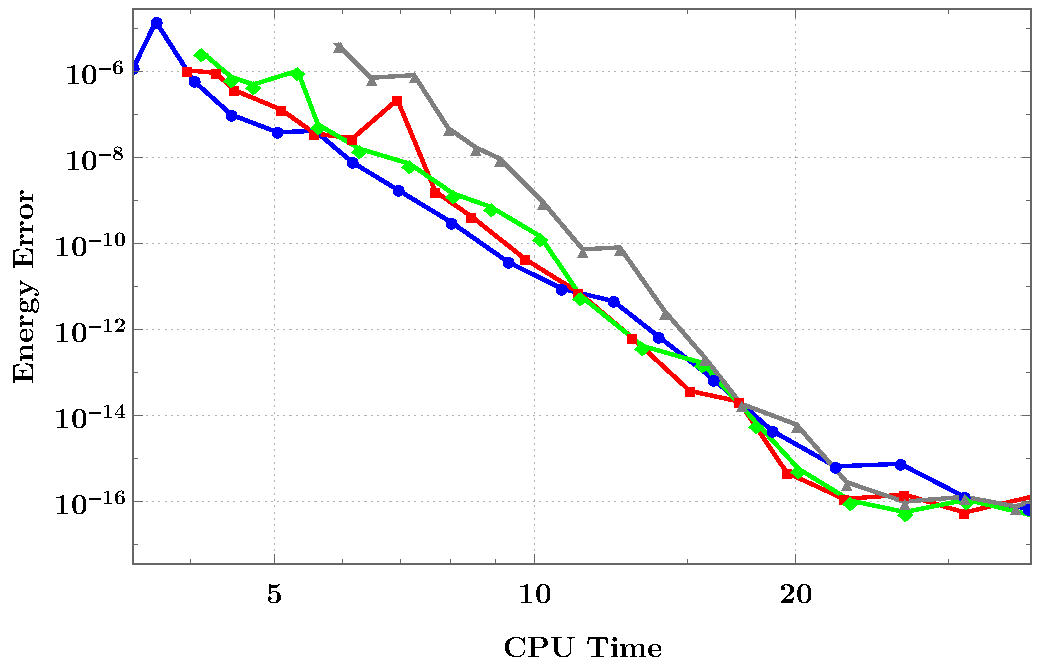
\includegraphics[width=.45\textwidth]{esperimentua811}}
&
\subfloat[ Exekuzio paraleloa.]
{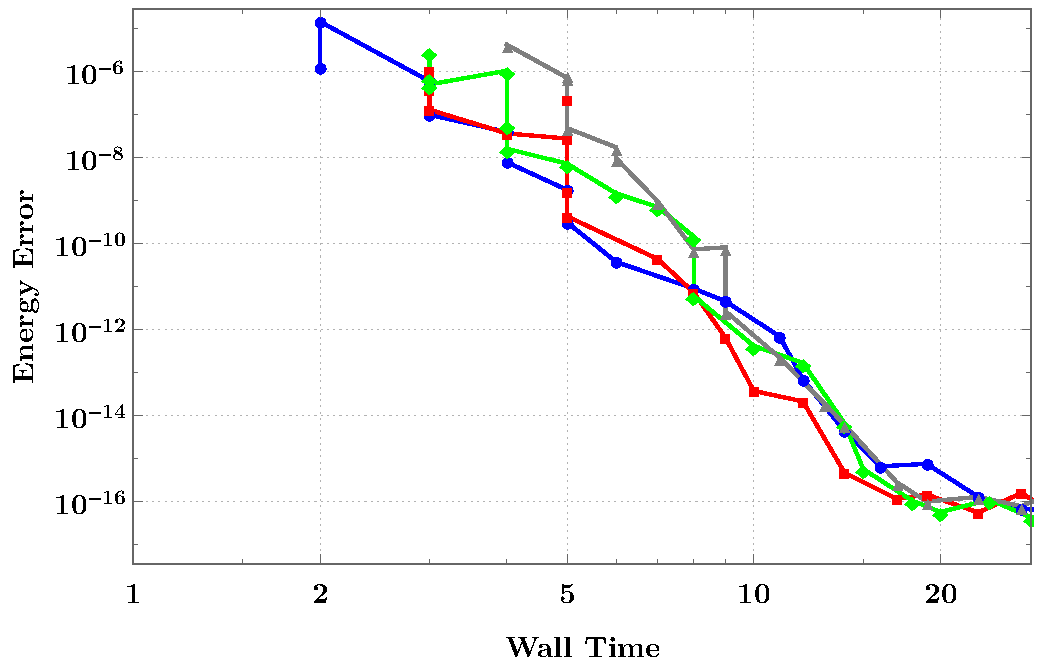
\includegraphics[width=.45\textwidth]{esperimentua813}}
%\subfloat[Exekuzio paraleloa (hariak=$2$):Wall Time.]
%{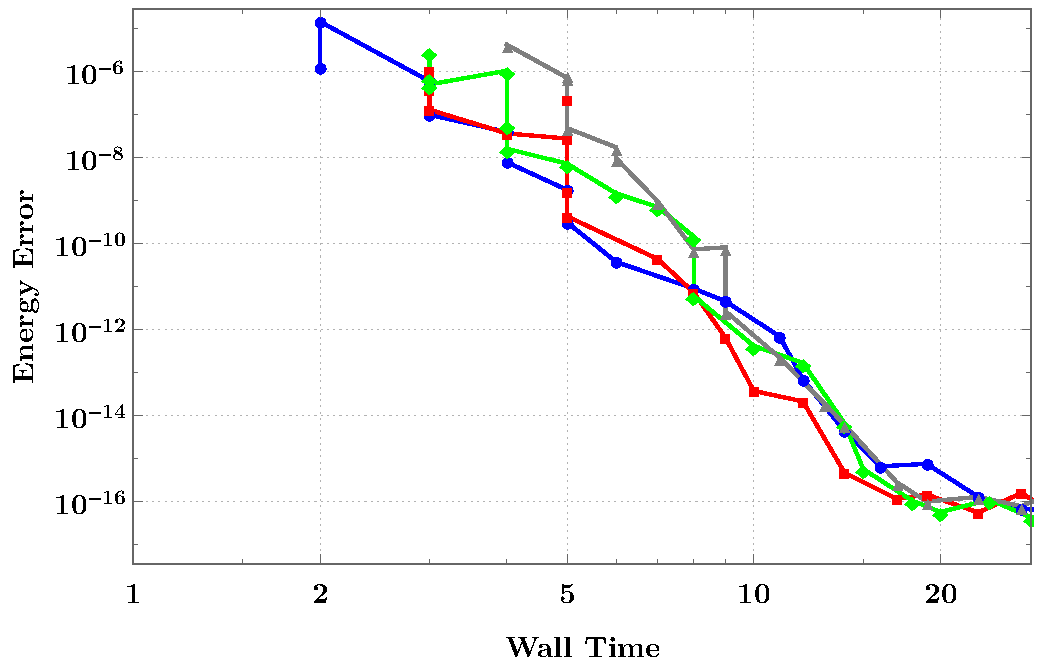
\includegraphics[width=.5\textwidth]{esperimentua813}}
%&
%\subfloat[Exekuzio paraleloa (hariak=$4$): Wall Time.]
%{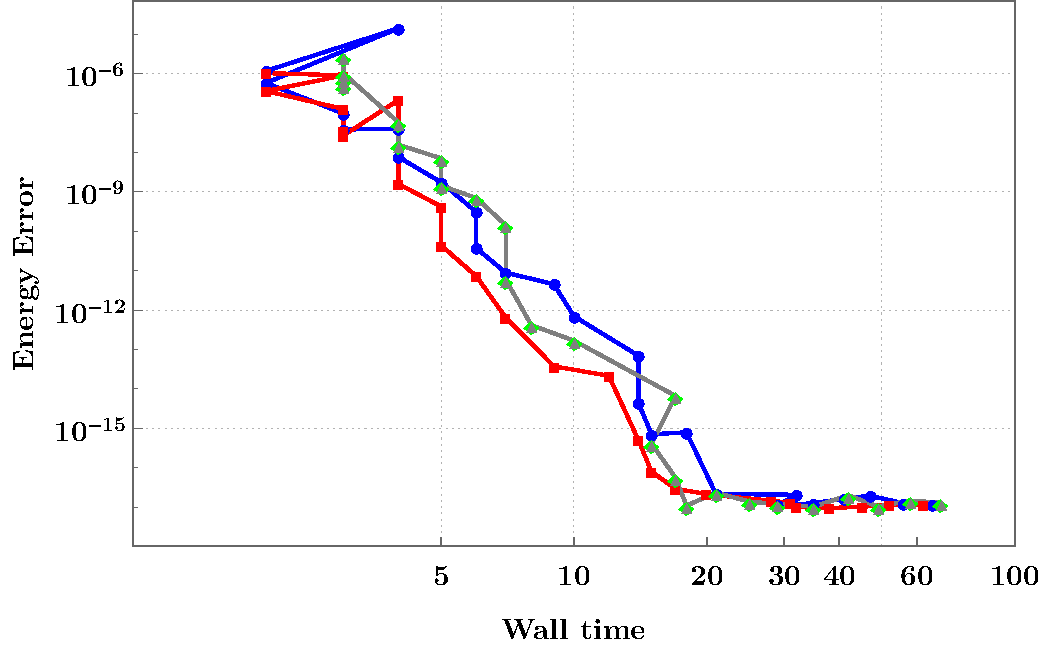
\includegraphics[width=.5\textwidth]{esperimentua814}}
\end{tabular}
\caption[Gauss metodoen eraginkortasun konparaketa (CPU Time)]{\small 
Eraginkortasun grafikoak eskala logaritmiko bikoitzean irudikatu ditugu. Ardatz bertikalean, energiaren errore erlatibo maximoa eman dugu eta ardatz horizontalean,  CPU denbora (exekuzio paraleloan Wall-Time). (a)  konputazioa modu sekuentzialean egin dugu eta (b) modu paraleloan hari kopurua $2$ izanik. Irudi bakoitzean, Gauss metodoaren $s$ ataletako lau integrazio konparatu ditugu: $s=6$  urdinez, $s=8$ gorriz, $s=9$ berdez, eta $s=16$ grisez. }
\label{fig:esp81s}
\end{figure}

Exekuzio sekuentzialak eta exekuzio paraleloak aztertuz,  Gauss metodo eraginkorrena aukeratu nahi dugu. Horretarako, biribiltze errorea nagusitzen hasten den inguruko unean gertatutakoa aztertu dugu: $s=8,9,16$ metodoak, $s=6$ metodoa baino eraginkorragoak azaldu zaizkigu. $s=8,9,16$ metodoak beraien artean oso antzekoak izanik, $s=8$ ataleko Gauss metodoa aukeratu dugu. Bestalde, exekuzio paraleloa, sekuentziala baino eraginkorragoa da.

\subsection*{Energia errorea eta errore globalak.}

%$s=8$ metodoarentzat, birbiltze errorea hasten den uneko urrats luzera hartu dut: $k=12, \ h=10,667$. Kokapen errore erlatiboaren estimazioa, $h/2$ integrazioarekiko diferentzia gisa kalkulatu ditugu.
Atal honetan, $s=8$ ataleko Gauss metodoaren, \emph{CO1035} konposizio metodoaren eta \emph{ABAH1064} splitting metodoaren erroreak konparatu ditugu.  Hiru errore mota ezberdin aztertu ditugu: energia errorea; kokapen eta abiaduren erroreen estimazioak; orbita eliptikoaren erdi-ardatz nagusiaren (\emph{semi-axis}) eta eszentrikotasunaren erroreen estimazioak. Gauss metodoa $h=10.63$ urrats luzerarekin integratu dugu eta  \emph{CO1035}, \emph{ABAH1064} metodoak $h=4.76$ urrats luzerarekin.

\subsubsection*{Energiaren eboluzioa}


\ref{fig:esp83}~irudian, lau integrazioen energiaren errore erlatiboaren eboluzioa erakutsi ditugu. Batetik, Gauss metodoa $64$-biteko (\emph{double}) proiekzioarekin eta $80$-biteko (\emph{double}) proiekzioarekin konputatutako integrazioak. Bestetik, \emph{CO1035} konposizio eta \emph{ABAH1064} splitting metodoen integrazioak. Proiekzioa $80$-biteko doitasunarekin kalkulatzerakoan, energiaren errorea modu esanguratsuan txikitzea lortu dugu. Aipagarria da ere, Gauss metodoa $80$-biteko proiekzioaren integrazioa, \emph{ABAH1064} splitting metodoarekin alderatuz, energia errorea txikiagoa dela.

\begin{figure}[h!]
\centering
\begin{tabular}{c c}
\subfloat[Gauss metodoa ($s=8$).]
{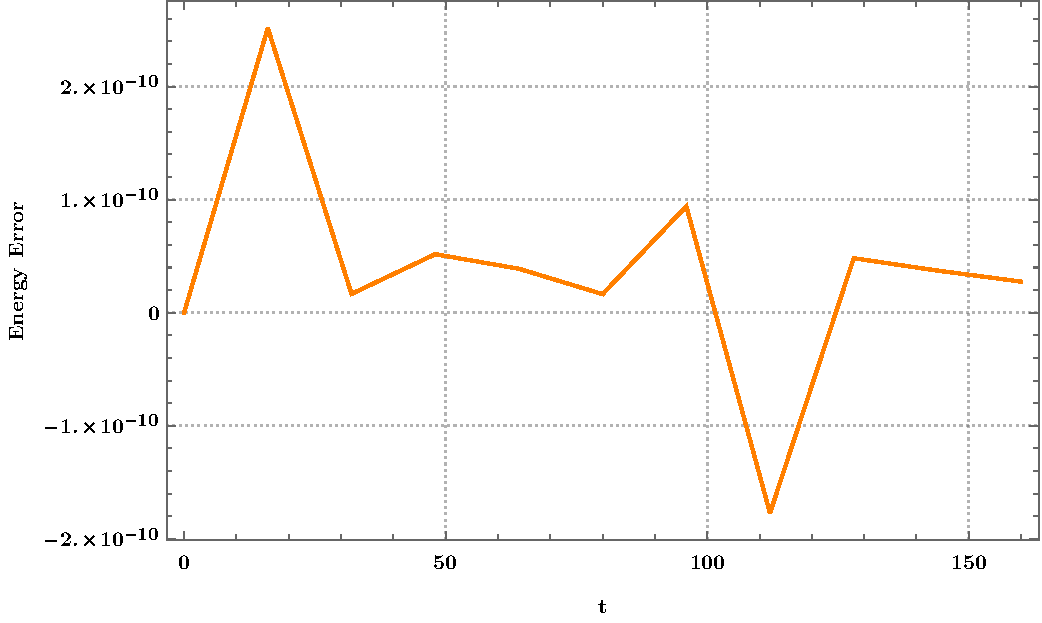
\includegraphics[width=.45\textwidth]{esperimentua831}}
&
\subfloat[ABAH1064 eta CO1035]
{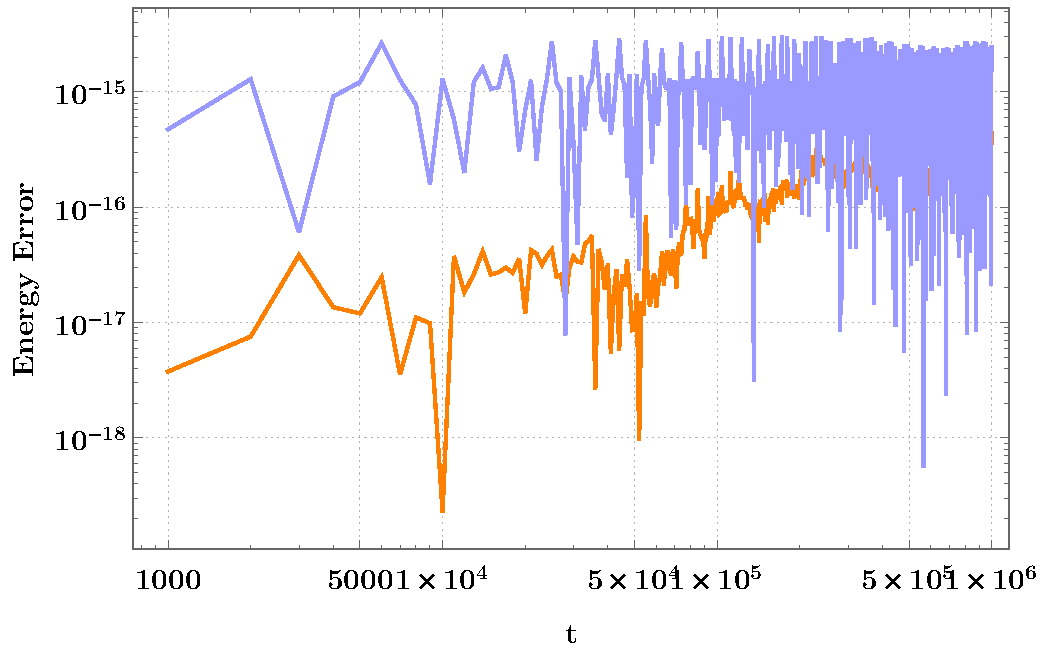
\includegraphics[width=.45\textwidth]{esperimentua832}}
\end{tabular}
\caption[Energia errorea]{\small Energia errorearen eboluzioa lau integrazio metodoetarako erakutsi dugu. Ezkerreko irudian, $s=8$ ataletako Gauss metodoaren $h=10,667$ urrats luzerarekin egindako integrazioak erakutsi ditugu: proiekzioa $80$-biteko \emph{long double} doitasunarekin (laranjaz) eta proiekzioa $64$-biteko \emph{double} doitasunarekin (urdinez). Eskuineko irudian, splitting/konposizio metodoak erakutsi ditugu: ABAH1064 (laranjaz) eta CO1035(urdinez)}
\label{fig:esp83}
\end{figure}


\subsubsection*{Kokapen eta abiadura erroreen estimazioak}


\ref{fig:esp84}~irudian, Gauss ($s=8$) eta \emph{ABAH1064} metodoentzako, kokapen eta abiaduraren erroreen estimazioak erakutsi ditugu. Erroreak estimatzeko, urrats txikiagoako integrazioaren soluzioarekiko diferentzia gisa kalkulatu dugu. 
Gauss metodoaren integrazioan, urrats luzera handiago erabili arren, barne-planeten kokapen eta abiaduren errore estimazioak, \emph{ABAH1064} splitting metodoaren integrazioan baino txikiagoak izan dira. 

\begin{figure}[h!]
\centering
\begin{tabular}{c c}
\subfloat[Gauss metodoa (kokapen errorea)]
{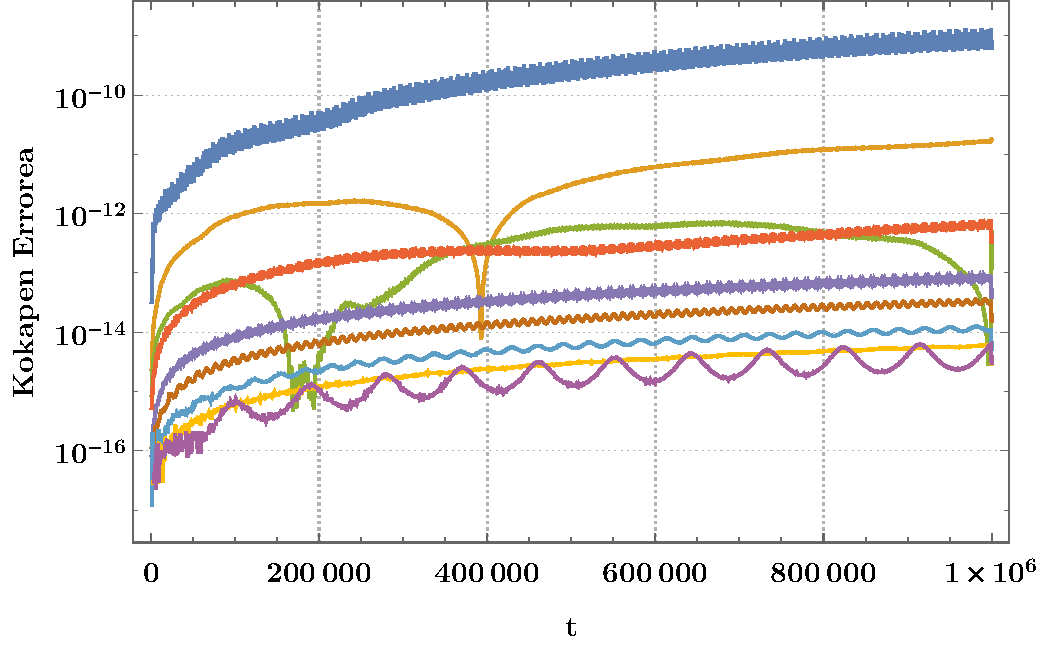
\includegraphics[width=.45\textwidth]{esperimentua841}}
&
\subfloat[Gauss metodoa (abiadura errorea)]
{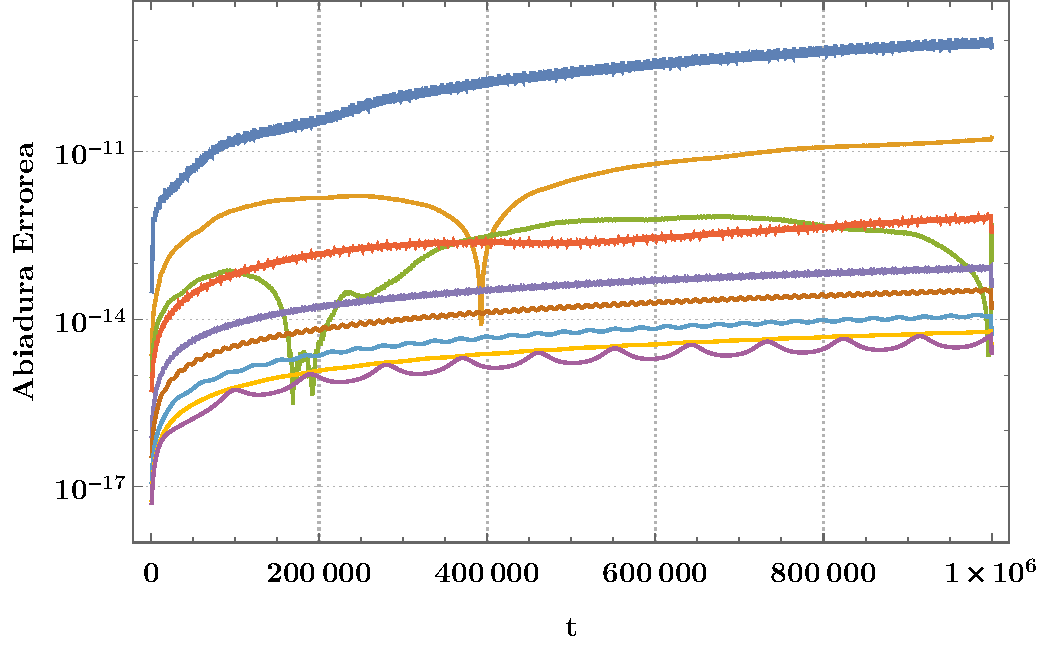
\includegraphics[width=.45\textwidth]{esperimentua842}}
\\
\subfloat[ABAH1064 (kokapen errorea)]
{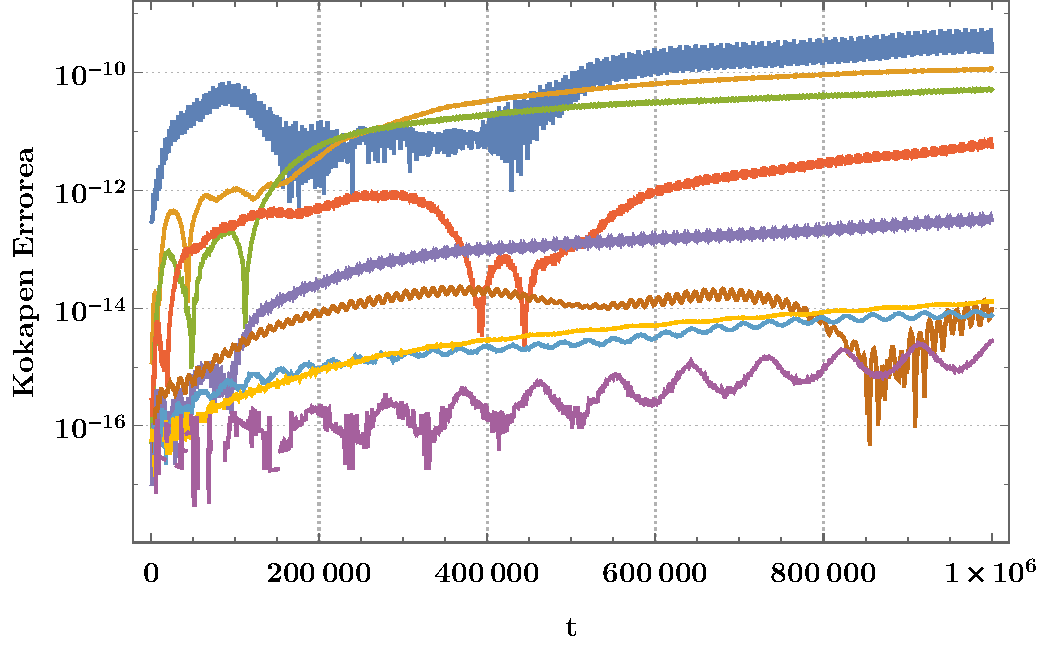
\includegraphics[width=.45\textwidth]{esperimentua843}}
&
\subfloat[ABAH1064 (abiadura errorea)]
{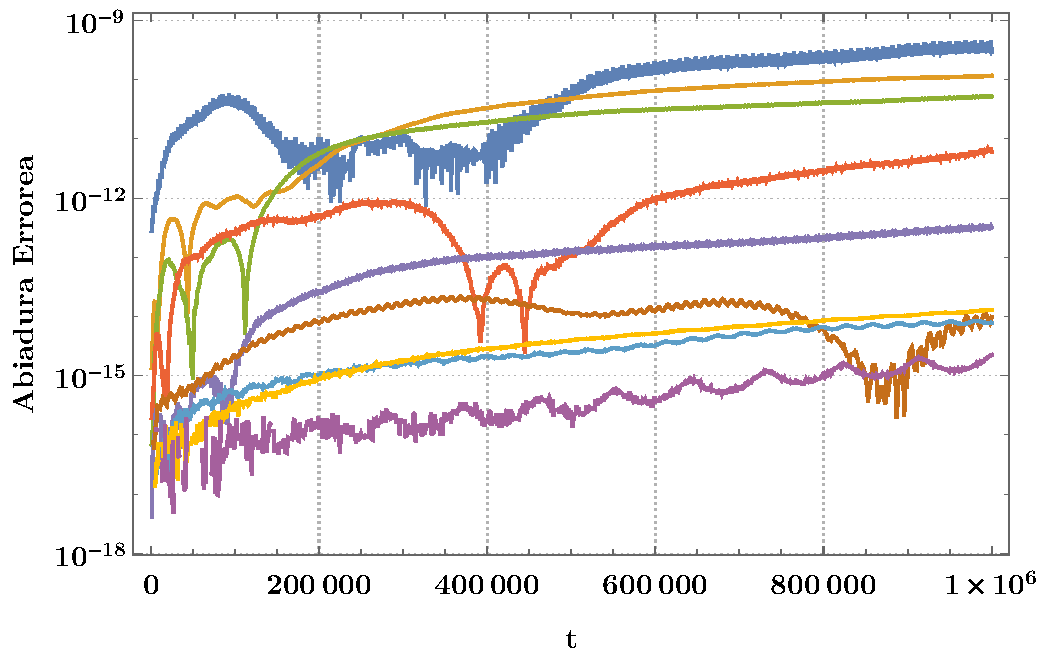
\includegraphics[width=.45\textwidth]{esperimentua844}}
\end{tabular}
\caption[Kokapen eta abiadura erroreak]{\small Kokapen eta abiaduraren erroreen estimazioak erakutsi ditugu. (a) eta (b) irudietan, $s=8$ ataletako Gauss metodoaren errore estimazioak eman ditugu, $h=10,667$ urrats luzera aplikatutako integrazioarentzat. (c) eta (d) irudietan, \emph{ABAH1064} splitting metodoaren errore estimazioak eman ditugu, $h=4.76$ urrats luzera aplikatutako integraziorentzat. Kolore bakoitza planeta bakoitzari dagokion errorea da: Merkurio (urdin ilunez), Artizarra (marroi argiz), Lurra (berdez), Marte (gorriz), Jupiter (more argiz), Saturno (marroi ilunez), Urano (urdin argiz), Neptuno (laranja argiz), Pluto (morez)}
\label{fig:esp84}
\end{figure}


\subsubsection*{Eszentrikotasun eta erdi-ardatza nagusiaren erroreen estimazioak}


Planeten mugimendu orbitala, eliptikoa da. Orbitaren propietateak finkatzen dituzten bi konstante hauen erroreen estimazioa kalkulatuko dugu: 
\begin{enumerate}
\item $a$ erdi-ardatz nagusia (\emph{semi-axis}) izeneko konstantea, orbita eliptikoaren tamaina definitzen duena.
\item $e$ eszentrikotasuna konstantea, orbita eliptikoaren forma finkatzen duena. 
\end{enumerate} 

\ref{fig:esp87}~irudian, bai Gauss metodoarentzat, bai \emph{ABAH1064} splitting metodoarentzat, $a$ erdi-ardatz nagusiaren eta $e$ eszentrikotasun erroreak, kokapen eta abiaduren erroreak baino txikiagoak dira. Honek esan nahi du, integrazioaren orbitaren forma mantentzen dela eta errorea, orbitaren fasean nagusitzen dela. Esperimentu honetan ere, Gauss metodoaren erroreak, \emph{ABAH1064} spliting metodoarenak baina txikiagoak dira.   

\begin{figure}[h!]
\centering
\begin{tabular}{c c}
\subfloat[Gauss maetodoa (erdi-ardatz nagusiaren errorea)]
{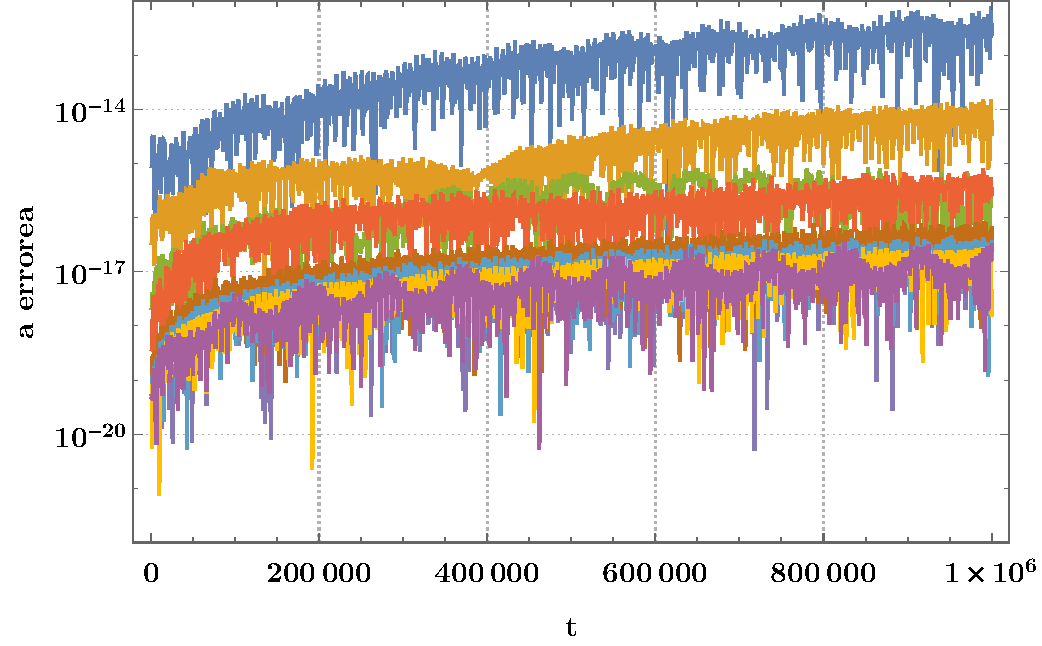
\includegraphics[width=.45\textwidth]{esperimentua871}}
&
\subfloat[Gauss maetodoa (eszentrikotasunaren errorea)]
{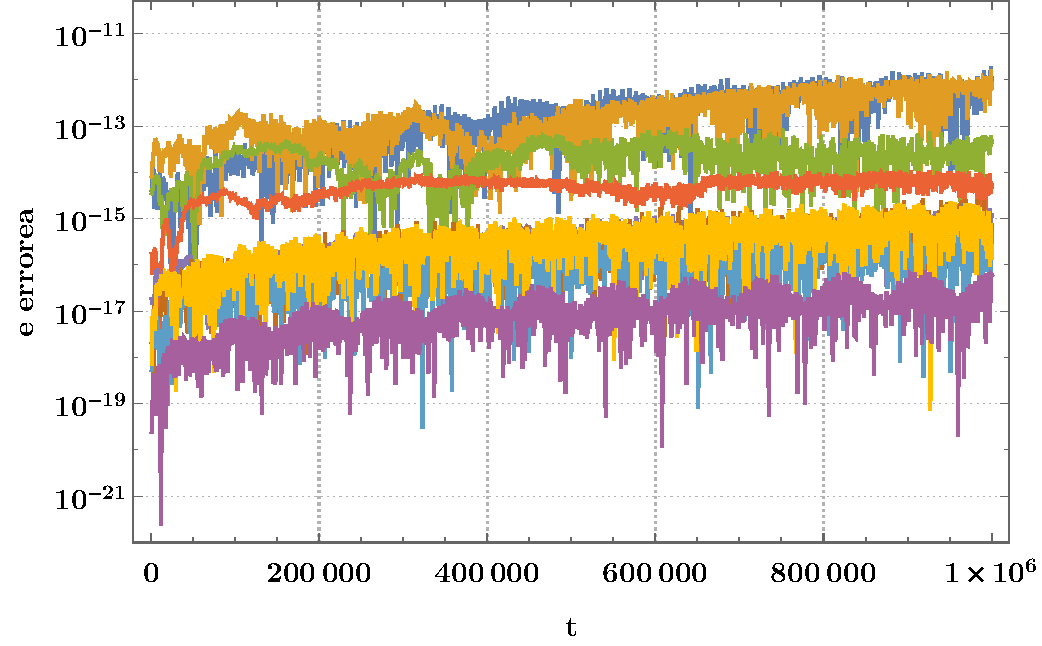
\includegraphics[width=.45\textwidth]{esperimentua872}}\\
\subfloat[ABAH1064 (erdi-ardatz nagusiaren errorea)]
{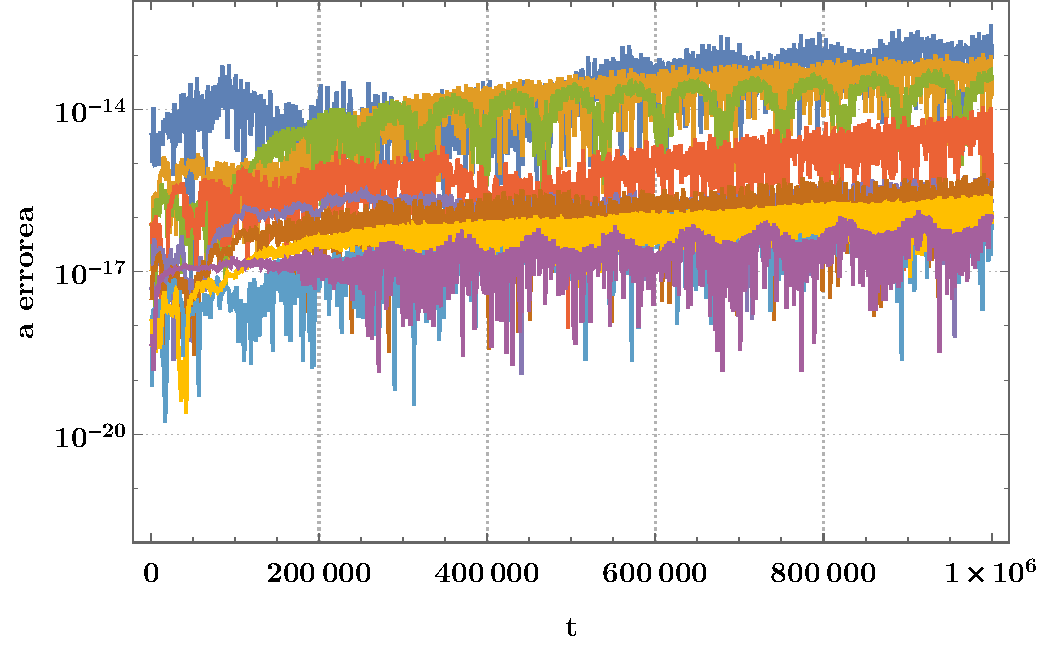
\includegraphics[width=.45\textwidth]{esperimentua873}}
&
\subfloat[ABAH1064 (eszentrikotasunaren errorea)]
{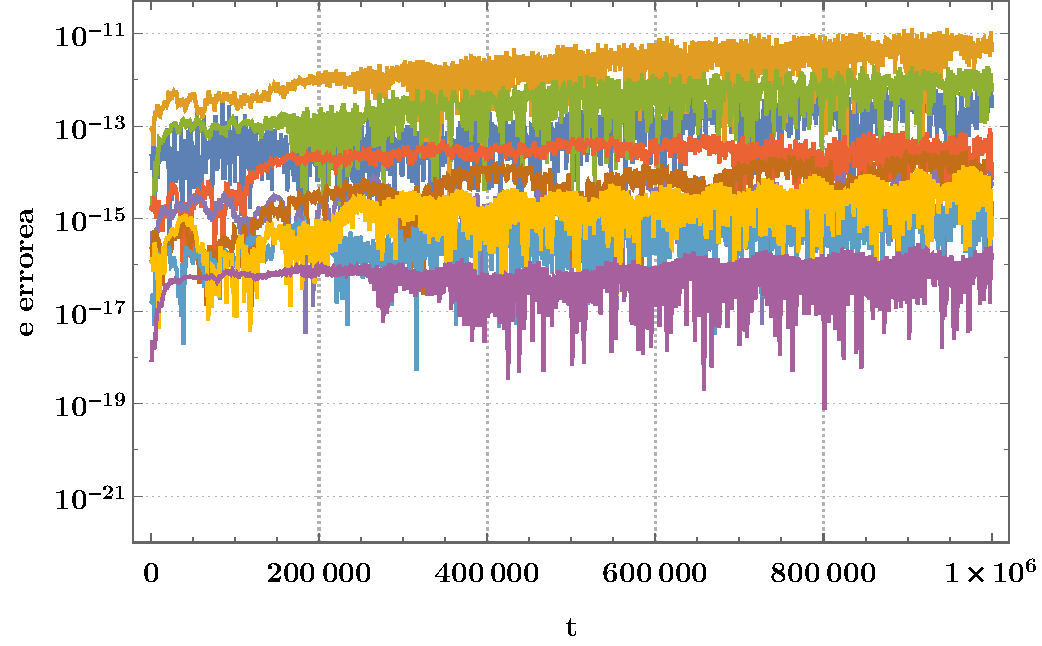
\includegraphics[width=.45\textwidth]{esperimentua874}}
\end{tabular}
\caption[Erdi-ardatz nagusiaren eta eszentrikotasunaren errorea]{\small \small Orbita eliptikoaren $a$ erdi-ardatz nagusiaren  eta $e$ eszentrikotasunaren erroreen estimazioak erakutsi ditugu. (a) eta (b) irudietan, $s=8$ ataletako Gauss metodoaren errore estimazioak eman ditugu, $h=10,667$ urrats luzerarekin integratuz. (c) eta (d) irudietan, \emph{ABAH1064} Splitting metodoaren errore estimazioak eman ditugu, $h=4.76$ urrats luzerarekin integratuz. Kolore bakoitza planeta bakoitzari dagokion errorea da: Merkurio (urdin ilunez), Artizarra (marroi argiz), Lurra (berdez), Marte (gorriz), Jupiter (more argiz), Saturno (marroi ilunez), Urano (urdin argiz), Neptuno (laranja argiz), Pluto (morez)}
\label{fig:esp87}
\end{figure}

\subsection*{Biribiltze errorea.}


Hirugarren esperimentu honetan, biribiltze errorea ilustratzeko esperimentua egin dugu eta horretarako, momentu angeluarraren errore erlatiboaren eboluzioan oinarritu gara. % Momentu angeluarraren trunkatze errorea beti zero da eta metodo sinplektikoek inbariante koadratikoak zehazki mantentzen dituzte. 
Lau faktore hartu behar dira kontutan. Kepler-en fluxuak, momentu angeluarra zehazki mantentzen du eta jatorrizko ekuazio diferentzialen inbariante koadratikoa da. Hori dela-eta, Kepler-en fluxuan oinarritutako aldagai aldaketarekin lortutako ekuazio diferentzialen inbariante koadratikoa da. Integratzeko Runge-Kutta metodo sinplektikoa aplikatu dugunez, inbariante koadratikoak zehazki mantentzen ditu eta beraz,  ikusten duguna biribiltze errorea da.

\ref{fig:esp85}~irudian, Gaussen $s=8$ ataletako metodoarekin, $h=9.0$ eta $h=10.63$ urrats luzerarekin integrazioen soluzioen momentu angeluarraren errorea erakutsi dugu eta espero bezala, biribiltze errorea zein den erakusten dute.


\begin{figure}[h!]
\centering
\begin{tabular}{c c}
\subfloat[Momentu angeluarra $h=9.0$.]
{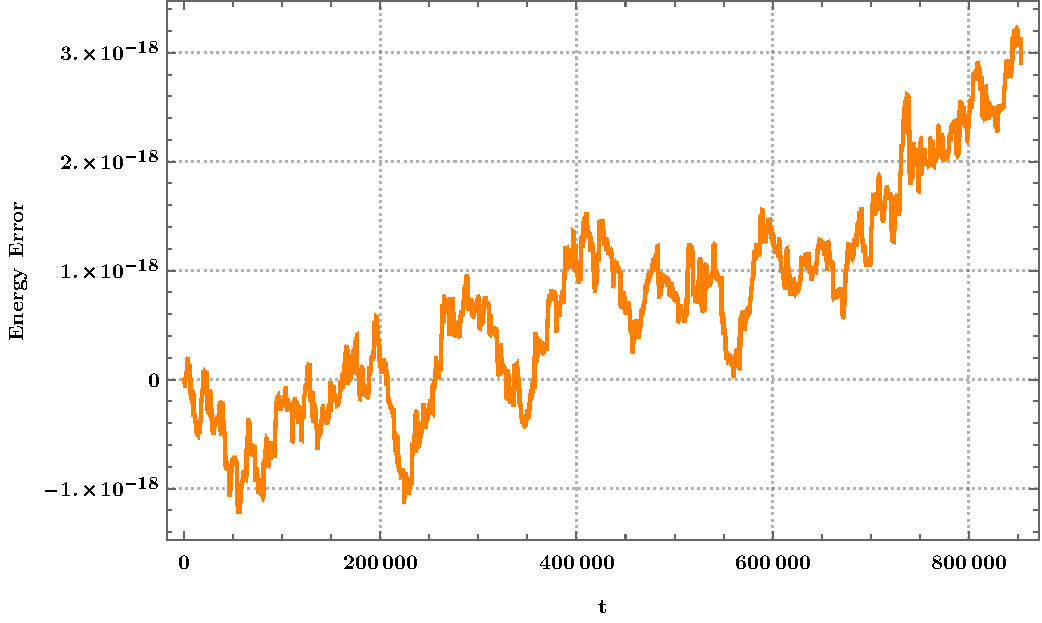
\includegraphics[width=.45\textwidth]{esperimentua851}}
&
\subfloat[Momentu angeluarra $h=10.63$]
{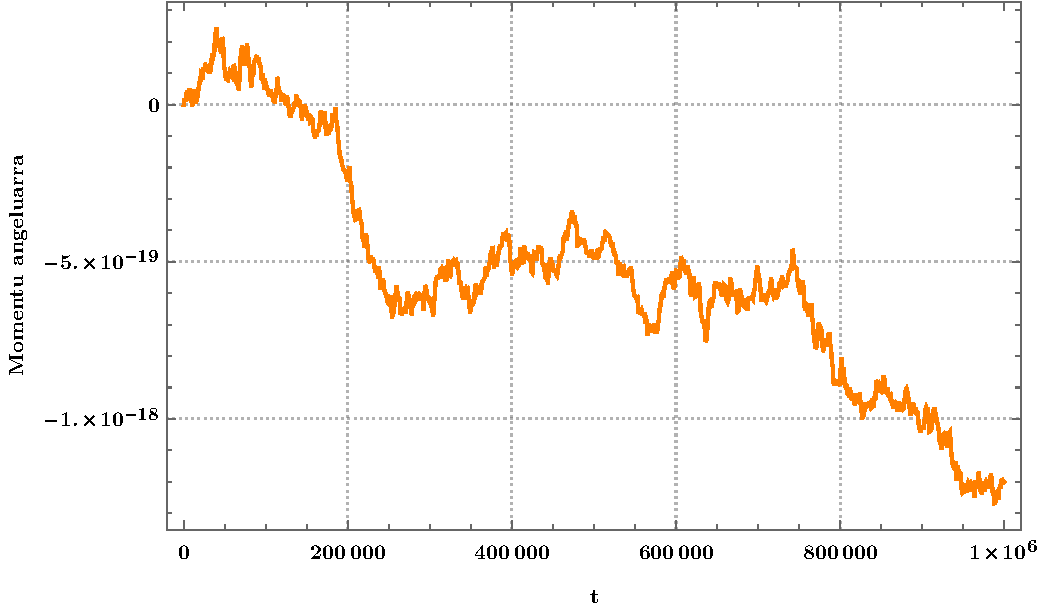
\includegraphics[width=.45\textwidth]{esperimentua852}}
\end{tabular}
\caption[Momentu angeluarra]{\small Momentu angeluarraren errore erlatiboaren eboluzioa erakutsi dugu. Gaussen $s=8$ ataletako metodoa integratu dugu $h=9.0$ eta $h=10.63$ urrats luzerarekin. }
\label{fig:esp85}
\end{figure}



\subsection*{Eraginkortasun konparaketa.}


Atal honetan, Gauss metodoa eta konposizio/splitting metodoen arteko eraginkortasunaren konparaketa egin dugu. \ref{fig:esp82a}~irudian, eraginkortasuna, ekuazio diferentzialaren ebaluazio kopuruaren arabera neurtu dugu. Gure inplementazio berriak, \emph{ABAH1064} splitting metodoak baino doitasun txikiagoa lortzen du. Etorkizuneko inplementazioaren konputazioa, $80$-biteko doitasunean eta proiekzioa, $128$-biteko doitasunean egin daiteke: era honetan, bien arteko koxka handiago izango da.
   

\begin{figure} [h!]
\centerline{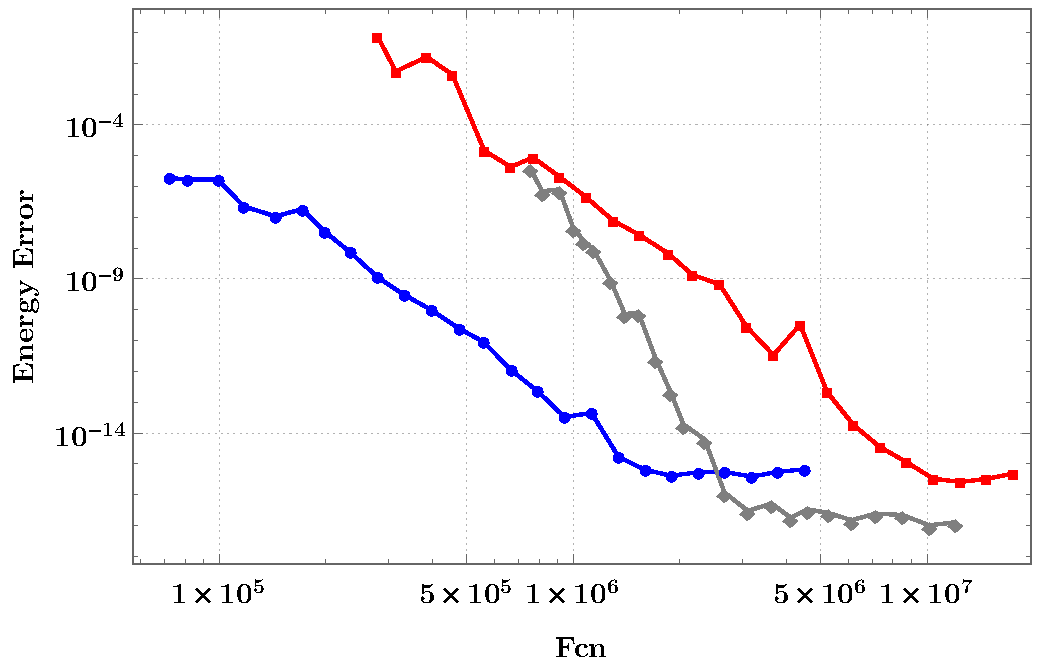
\includegraphics [width=8cm, height=6cm] {esperimentua822}}
\caption[Metodo sinplektikoen eraginkortasun grafikoa (FCN)]{\small Eraginkortasun grafikoa, eskala logaritmiko bikoitzean irudikatu dugu. Ardatz bertikalean, energiaren errore erlatibo maximoa eman dugu eta ardatz horizontalean, ekuazio diferentzialen ebaluazio kopurua (FCN).  Hiru integrazio metodo konparatu ditugu: $s=6$ Gauss metodoa grisez, $ABAH1064$  urdinez eta $CO1035$ gorriz}
\label{fig:esp82a}
\end{figure} 

\ref{fig:esp82}~irudian, $s=8$ ataletako Gauss metodoa, modu sekuentzialean eta modu paraleloan exekutatu dugu. Eguzki-sistemaren eredu sinplearen integraziorako, splitting metodoak oso eraginkorrak azaldu zaizkigu. Gauss metodoaren exekuzioa paralelizatzeak abantaila erakusten du baina hala ere, splitting metodoak eraginkorragoak dira.

Dena den, eredu errealistagoak (gorputz kopurua handitzen delako edota erlatibitate efektua kontutan hartzen delako) integratzeko, Gauss metodoak eraginkorragoak bilakatzea espero da. Splitting metodoen konputazioak, modu trinkoan kalkulatu behar dira, hau da, atalen konputazioak sekuentzialki exekutatzen dira eta  ez ditu konputazio aldaerarik onartzen. Gauss metodoaren ekuazio inplizituak ebazteko, ordea, teknika ezberdinak konbina daitezke eta eraginkortasuna hobetzeko aukera asko eskaintzen dizkigu. Adibidez, iterazio gehienak problemaren eredu sinple batekin, doitasun baxuan kalkula daitezke  \cite{Beylkin2014} eta bukaerako iterazio pare bat eredu osoarekin, doitasun altuan. Gauss metodoaren $s$-ataletako funtzioen ebaluazioak  modu paraleloan exekutatu daitezke eta eguzki-sistemaren eredu konplexuagoa aplikatzen den neurrian, paralelizazioak abantaila handiagoa suposatuko du.



\begin{figure}[h!]
\centering
\begin{tabular}{c c}
\subfloat[Exekuzio sekuentziala.]
{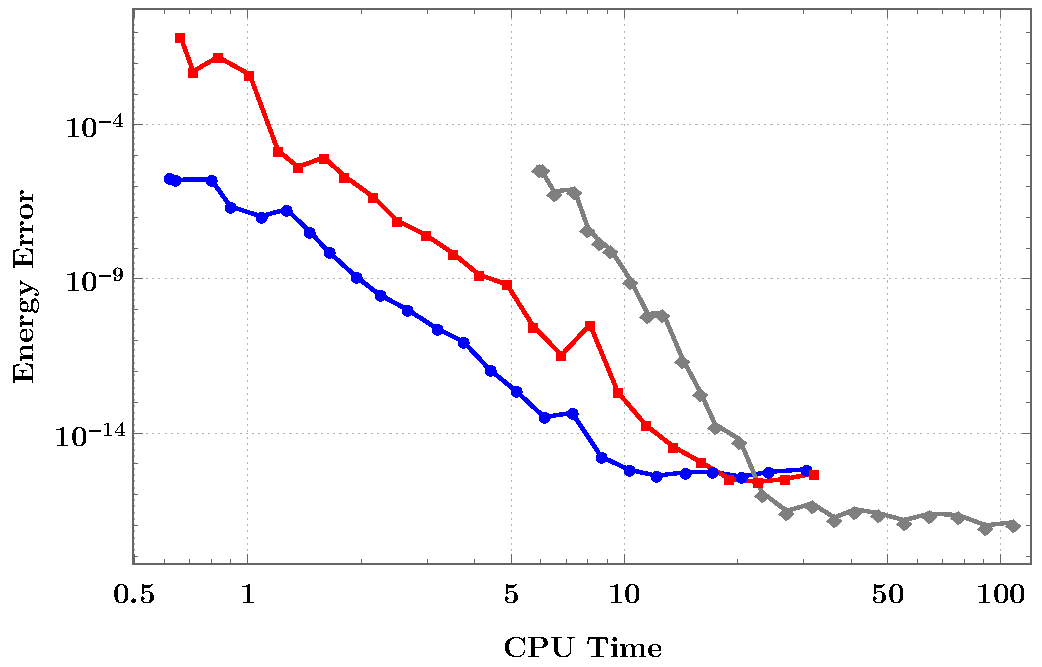
\includegraphics[width=.45\textwidth]{esperimentua821}}
&
\subfloat[Exekuzio paraleloa.]
{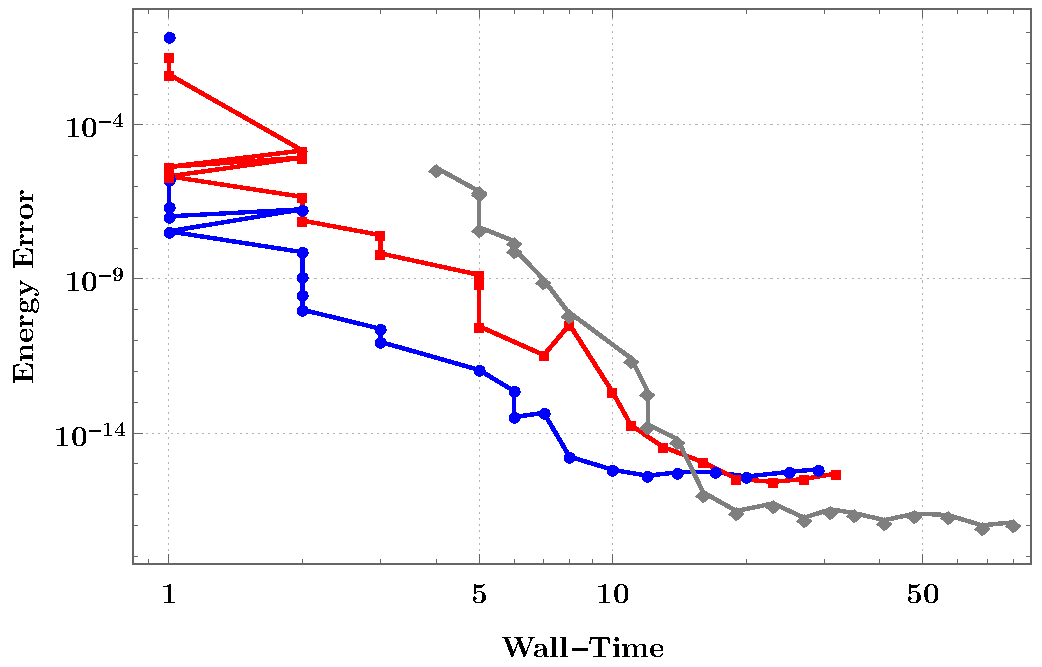
\includegraphics[width=.45\textwidth]{esperimentua823}}
%\subfloat[Exekuzio paraleloa (hariak=$2$) Wall Time.]
%{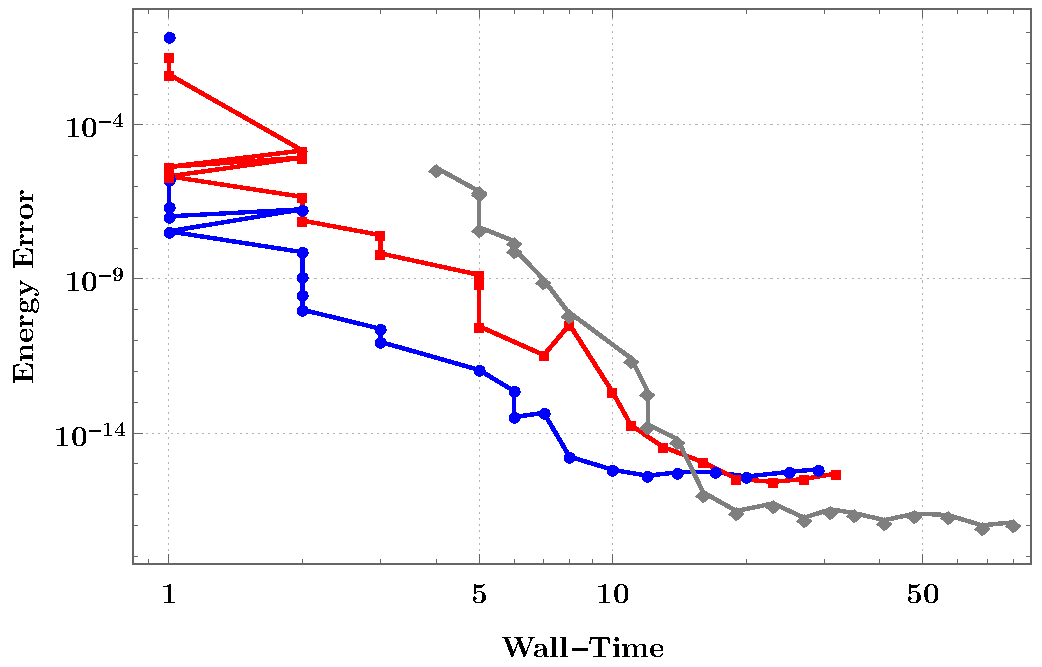
\includegraphics[width=.5\textwidth]{esperimentua823}}
%&
%\subfloat[Exekuzio paraleloa (hariak=$4$) Wall Time.]
%{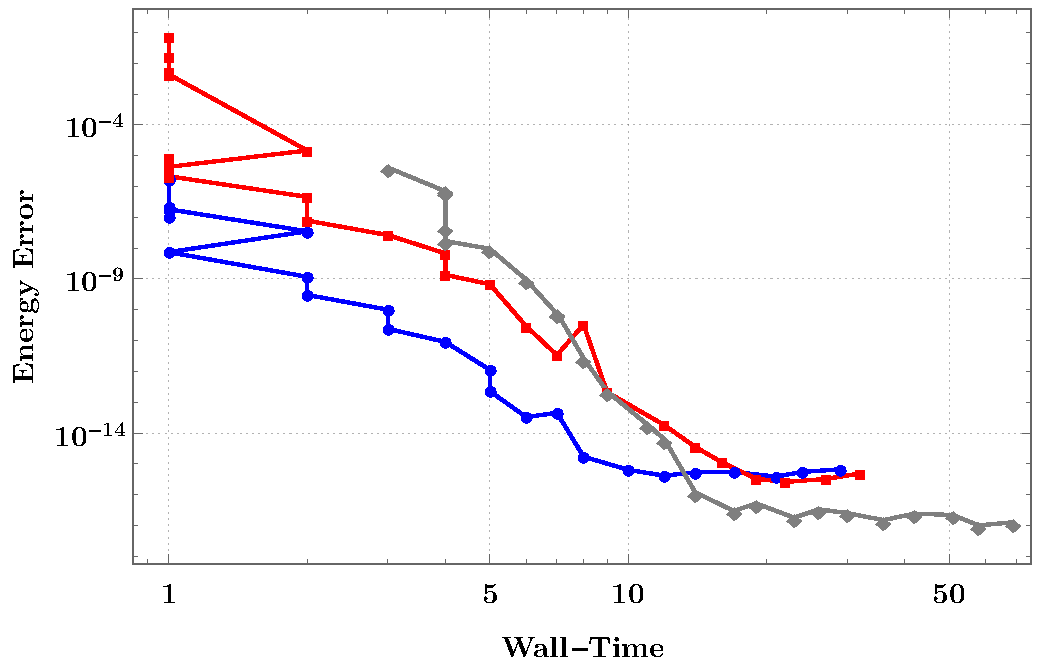
\includegraphics[width=.5\textwidth]{esperimentua824}}
\end{tabular}
\caption[Metodo sinplektikoen eraginkortasun grafikoa (CPU Time)]{\small 
Eraginkortasun grafikoak eskala logaritmiko bikoitzean irudikatu ditugu. Ardatz bertikalean, energiaren errore erlatibo maximoa eman dugu eta ardatz horizontalean,  CPU denbora (exekuzio paralelotan Wall-Time) erakutsi dugu. (a) konputazioa modu sekuentzialean egin dugu eta (b) modu paraleloan, hari kopurua $2$ izanik. Irudi bakoitzean,  hiru integrazio metodo konparatu ditugu: $s=6$ Gauss metodoa grisez, $ABAH1064$  urdinez eta $CO1035$ gorriz
}
\label{fig:esp82}
\end{figure}

%\begin{figure}[h!]
%\centering
%\begin{tabular}{c c}
%\subfloat[$s=16$ Exekuzio sekuentziala: CPU-denbora.]
%{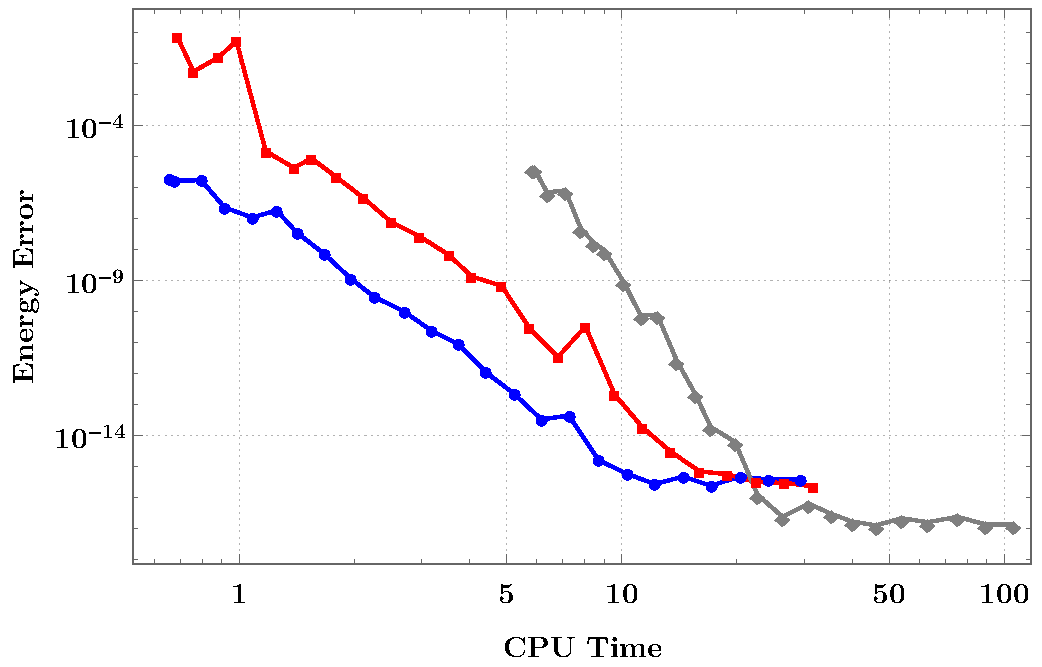
\includegraphics[width=.5\textwidth]{esperimentua861}}
%&
%\subfloat[$s=16$ Exekuzio sekuentziala:: FCN.]
%{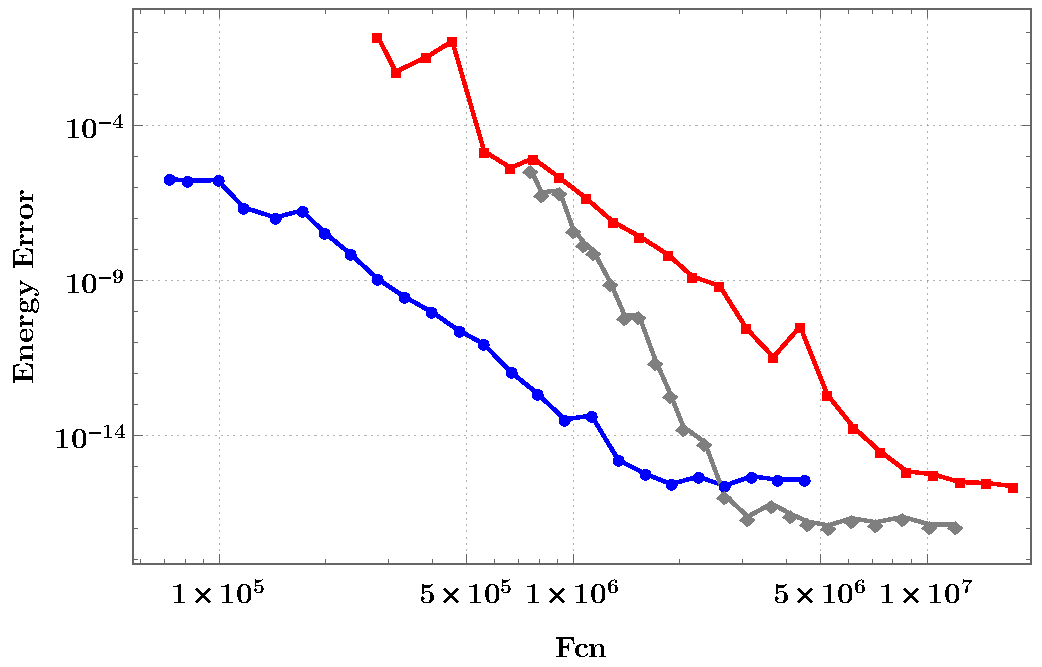
\includegraphics[width=.5\textwidth]{esperimentua862}}\\
%\subfloat[$s=16$ Exekuzio paraleloa: hariak=$2$.]
%{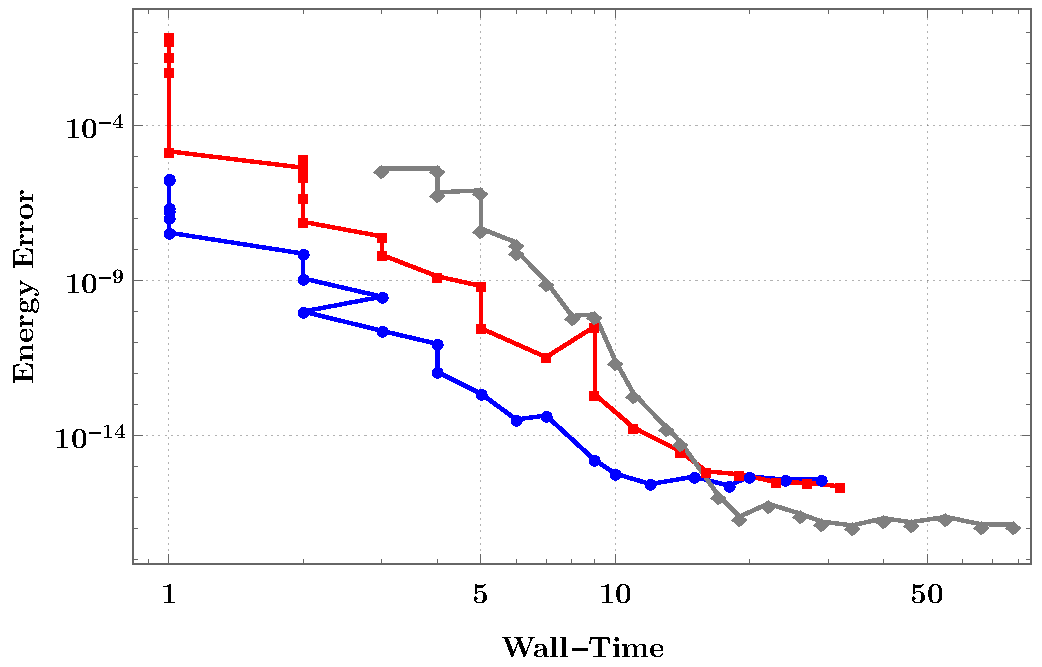
\includegraphics[width=.5\textwidth]{esperimentua863}}
%&
%\subfloat[$s=16$ Exekuzio paraleloa: hariak=$4$.]
%{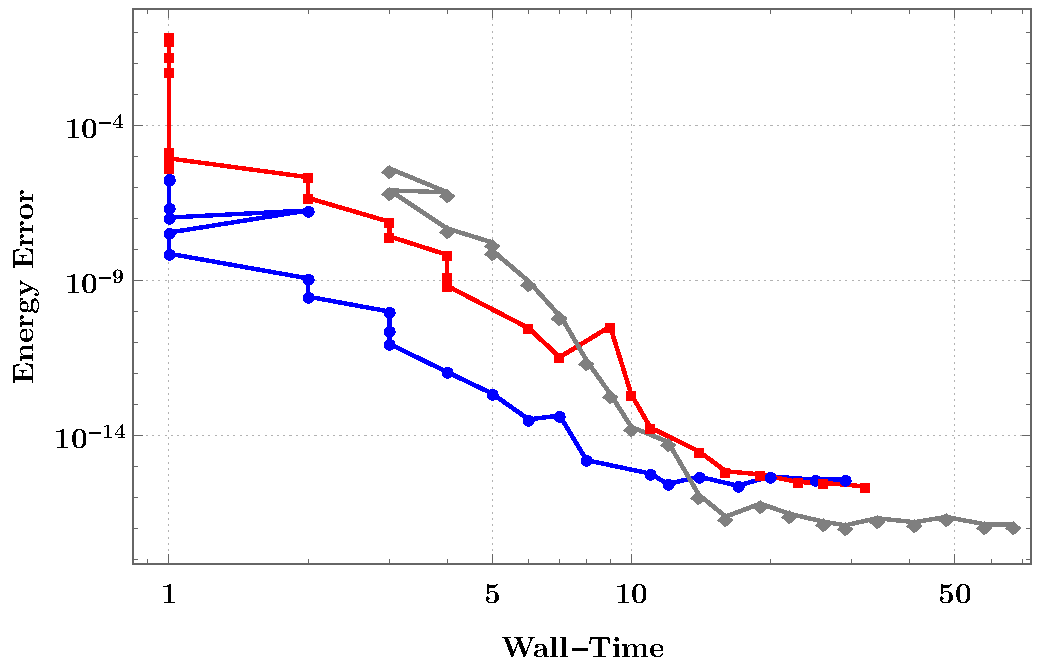
\includegraphics[width=.5\textwidth]{esperimentua864}}
%\end{tabular}
%\caption{\small 
%Eraginkortasun grafikoak irudikatu ditugu: ezkerrean energiaren errore maximoa, CPU denborarekiko; eskuinean ekuazio diferentzialen ebaluazio kopuruarekiko (FCN). Lau integrazio metodo konparatu ditugu: $ABAH1064$  urdinez, $CO1035$ gorriz,  eta \emph{IRKFLUXU} grisez}
%\label{fig:esp82}
%\end{figure}


\section{Laburpena.}


Kapitulu honetan, eguzki-sistemaren integraziorako inplementazio berri bat aurkeztu dugu. Inplementazio berria, egungo metodo sinplektiko eraginkorrenekin alderatu dugu eta emaitzak, baikorrak izateko modukoak iruditu zaizkigu. Oinarrizko azterketa egin badugu ere, agerian geratu da, metodoak etorkizunean izan ditzakeen potentziala. Dudarik gabe, etorkizun hurbilean azterketa sakonagoa egin beharko litzateke, metodoaren propietate onak baieztatzeko. Horien artean, honako ideia aipatuko ditugu:
\begin{enumerate}
\item $80$-biteko doitasuneko (\emph{long double}) integrazioaren konputazioa: kasu honetan, proiekzioa $128$-biteko doitasunean egitea komeniko litzateke. 
\item Kepler fluxuaren inplementazioaren hobekuntzak: oraingo inplementazioaren iterazio guztietan, ez dugu aurreko iterazioen informazio erabiltzen. Iterazio berri baten kalkuluan, aurreko iterazioren egoeretatik abiatuta, nahikoa izango litzateke fluxuaren iterazio bakarra egitea.  
\item Eguzki sistemaren eredu konplexuago batekin (Ilargia eta zenbait asteroide, erlatibitate efektua, eguzkiaren atxatamendua,\dots), Gauss metodoa eraginkorragoa bilakatzea espero da. Eguzki-sistemaren eredu konplexuago, aplikatzen den neurrian paralelizazioak abantaila handiagoa suposatuko du. Era berean, iterazio gehienak problemaren eredu sinple batekin, doitasun baxuan kalkula daitezke eta bukaerako iterazio pare bat eredu osoarekin, doitasun altuan.
\item Eraginkortasuna hobetzeko, Jacobiarraren hurbilpen sinple baten erabilera (puntu finkoaren eta Newton-en arteko algoritmo eraginkorra).  
\end{enumerate}    

Eguzki-sistema eredu konplexuetan, Kleperiarrak ez diren indarrak aplika daitezke. Aldagai hauen konbergentzia azkartzeko, Newton sinplifikatuaren iterazioan oinarritutako inplementazioa aplikatzea komeniko da.  

Azkenik, aipatu nahi dugu, inplementazioaren kodea, helbide honetan \url{https://github.com/mikelehu/IRK-SolarSystem} eskuragarri jarri dugula. 

